
%%%%%%%%%%%%%%%%%%%%%%%%%%%%%%%%%%%%%%%%%
% Beamer Presentation
% LaTeX Template
% Version 1.0 (10/11/12)
%
% This template has been downloaded from:
% http://www.LaTeXTemplates.com
%
% License:
% CC BY-NC-SA 3.0 (http://creativecommons.org/licenses/by-nc-sa/3.0/)
%
%%%%%%%%%%%%%%%%%%%%%%%%%%%%%%%%%%%%%%%%%

%----------------------------------------------------------------------------------------
%	PACKAGES AND THEMES
%----------------------------------------------------------------------------------------

\documentclass{beamer}

\mode<presentation> {

% The Beamer class comes with a number of default slide themes
% which change the colors and layouts of slides. Below this is a list
% of all the themes, uncomment each in turn to see what they look like.

%\usetheme{default}
%\usetheme{AnnArbor}
%\usetheme{Antibes}
%\usetheme{Bergen}
%\usetheme{Berkeley}
%\usetheme{Berlin}
%\usetheme{Boadilla}
%\usetheme{CambridgeUS}
%\usetheme{Copenhagen}
%\usetheme{Darmstadt}
%\usetheme{Dresden}
%\usetheme{Frankfurt}
%\usetheme{Goettingen}
%\usetheme{Hannover}
%\usetheme{Ilmenau}
%\usetheme{JuanLesPins}
%\usetheme{Luebeck}
\usetheme{Madrid}
%\usetheme{Malmoe}
%\usetheme{Marburg}
%\usetheme{Montpellier}
%\usetheme{PaloAlto}
%\usetheme{Pittsburgh}
%\usetheme{Rochester}
%\usetheme{Singapore}
%\usetheme{Szeged}
%\usetheme{Warsaw}

% As well as themes, the Beamer class has a number of color themes
% for any slide theme. Uncomment each of these in turn to see how it
% changes the colors of your current slide theme.

%\usecolortheme{albatross}
%\usecolortheme{beaver}
%\usecolortheme{beetle}
%\usecolortheme{crane}
\usecolortheme{dolphin}
%\usecolortheme{dove}
%\usecolortheme{fly}
%\usecolortheme{lily}
%\usecolortheme{orchid}
%\usecolortheme{rose}
%\usecolortheme{seagull}
%\usecolortheme{seahorse}
%\usecolortheme{whale}
%\usecolortheme{wolverine}

%\setbeamertemplate{footline} % To remove the footer line in all slides uncomment this line
%\setbeamertemplate{footline}[page number] % To replace the footer line in all slides with a simple slide count uncomment this line

%\setbeamertemplate{navigation symbols}{} % To remove the navigation symbols from the bottom of all slides uncomment this line
}

\usepackage{graphicx} % Allows including images
\usepackage{booktabs} % Allows the use of \toprule, \midrule and \bottomrule in tables
\usepackage{array}
\usepackage{tabularx}
\usepackage[backend=biber,style=apa]{biblatex}
\addbibresource{references.bib}
\usepackage{hyperref}
\usepackage{changepage}
\usepackage[hang,flushmargin]{footmisc}
\usepackage[normalem]{ulem}
\hypersetup{
	colorlinks,
    citecolor={blue!70!black},
	linkcolor={blue!70!black},
	urlcolor={blue!70!black}}

\usepackage{appendixnumberbeamer}
\usepackage{amsmath}
\usepackage{booktabs}      % For \toprule, \midrule, \bottomrule
\usepackage{threeparttable} % For tablenotes
\usepackage{tikz}
\usetikzlibrary{arrows.meta}

%\setbeamercolor{alerted text}{fg=red!70!black}    % warm alert
%\setbeamercolor{alerted text}{fg=orange!80!black} % another option
%\setbeamercolor{alerted text}{fg=cyan!60!black} 

\definecolor{AlertOrangeRed}{RGB}{255,69,0}
\definecolor{AlertDarkOrange}{RGB}{255,140,0}
\definecolor{AlertTomato}{RGB}{255,99,71}
\definecolor{AlertCoral}{RGB}{255,127,80}
\definecolor{AlertGold}{RGB}{255,215,0}
\definecolor{AlertYellowOrange}{RGB}{255,174,66}
\definecolor{AlertMagenta}{RGB}{255,0,255}
\definecolor{AlertVermilion}{RGB}{227,66,52}

% Set default alert color (global)
\setbeamercolor{alerted text}{fg=AlertOrangeRed}
\setbeamertemplate{navigation symbols}{}     % remove all navigation symbols
%\setbeamertemplate{footline}{}  \beamertemplatenavigationsymbolsempty


%----------------------------------------------------------------------------------------
%	TITLE PAGE
%----------------------------------------------------------------------------------------

\title[Sharing Data with the Taxman]{Sharing Data with the Taxman} % The short title appears at the bottom of every slide, the full title is only on the title page

\author[Kircali, Stantcheva and Weber] % Short author list for footer
{Tim Kircali\inst{1} \and Stefanie Stantcheva\inst{2} \and Matthias Weber\inst{1}}

\institute[] % Short institution list for footer
{
\inst{1} University of St.Gallen \\
\inst{2} Harvard University
}
{
\medskip

}

\date[St.Gallen, Nov 2025]{Dec 2025}%Talk w. Kurt Schmidheiny, 
 % Date, can be changed to a custom date

\begin{document}

\begin{frame}
\titlepage % Print the title page as the first slide
\end{frame}


\begin{frame}
\frametitle{Two Key Rationales to Support Information-Sharing}
\begin{enumerate}
    \item Information exchange is \alert{highly effective to reduce tax evasion} \parencite{kleven2011unwilling,pomeranz2015no,slemrod2017does}
    \vspace{0.5em}
    \item The IRS needs information exchange to \alert{prepopulate tax returns}.
\end{enumerate}
\vspace{2em}
Big (!) potential: 
\vspace{0.5em}
\begin{itemize}
    \item In the U.S. \$696B (15\%) taxes are not paid on time and \$606B (13\%) are never collected \parencite{IRS_TaxGap_2022_Pub5869}.
    \vspace{0.5em}
    \item An average individual taxpayer has 13 hours and about \$250 tax filing costs \parencite{IRS2022}. This reflects a total cost of approximately \$100 billion per year. 
\end{itemize}
\end{frame}

\begin{frame}
\frametitle{Questions}
Should the U.S. adopt more comprehensive information exchange? 
\begin{itemize}
    \item \cite{boning2025welfare}: Stronger tax enforcement is welfare increasing in the U.S. (here by tax audits).
    \item \cite{kleven2011unwilling,pomeranz2015no,slemrod2017does}: Information sharing is highly effective to enforce taxes. 
\end{itemize}
\vspace{1em}
Should the U.S. offer free tax software and prepopulated tax returns?
\begin{itemize}
    \item Tax filing costs are high. (\cite{IRS2022}) \\[0.2em]
    \item Many other countries already offer these services.
\end{itemize}
\vspace{1em}
\begin{itemize}
    \item[$\Rightarrow$] \alert{Research generally says yes to policies.} 
    \item[$\Rightarrow$] \alert{But what do people think about them?}
\end{itemize}
\end{frame}

\begin{frame}{Survey to Measure (and Understand!) Policy Support }
\begin{columns}[T] % align columns at the top
  \begin{column}{0.5\textwidth} % left side for text
    \begin{itemize}
    \item Questions addressed to uncover the "invisible"
    \begin{itemize}
        \item Knowledge \& Perceptions
        \item Considerations \& Beliefs
        \item Policy support
    \end{itemize}
    \vspace{1em} 
    \item Provide \alert{policy-related information}
    \begin{itemize}
        \item Analyze how factors and considerations shape policy support
    \end{itemize}
    \end{itemize}
  \end{column}
  
  \begin{column}{0.45\textwidth} % right side for image
    \centering
    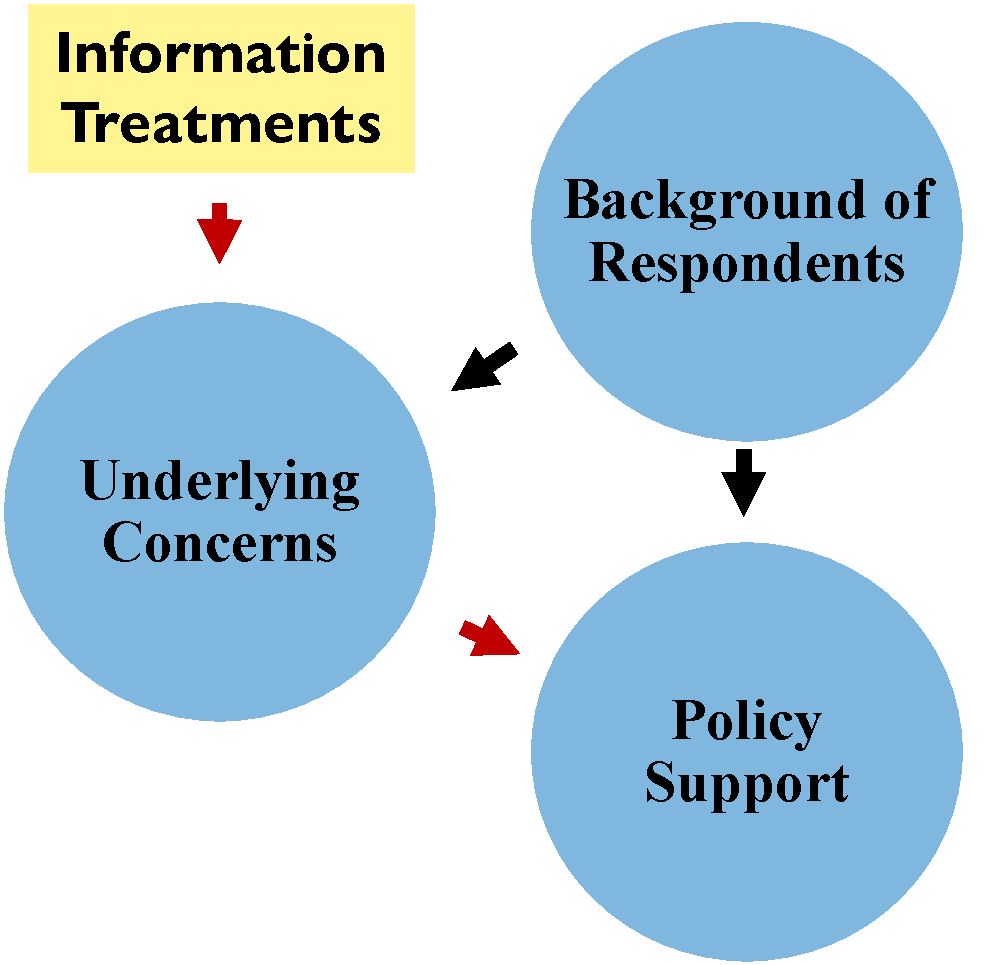
\includegraphics[width=\linewidth]{Figures_Slides/Estimation_Strategy.pdf}
  \end{column}
\end{columns}
\end{frame}

\begin{frame}{Focus on Four Considerations}
\begin{columns}[T] % align columns at the top
  \begin{column}{0.45\textwidth} % left side for text
  We concentrate on four key considerations:
  \vspace{1em}
    \begin{itemize}
        \item Tax Evasion and Government Revenue
        \vspace{0.25em}
        \item Fairness and inequality
        \vspace{0.25em}
        \item Filing Costs
        \vspace{0.25em}
        \item Data privacy
        \vspace{1em}
        \item[$\Rightarrow$] \alert{We provide respondents with information that directly addresses these considerations.}
    \end{itemize}
  \end{column}
  
  \begin{column}{0.45\textwidth} % right side for image
    \centering
     \vspace{-1em}     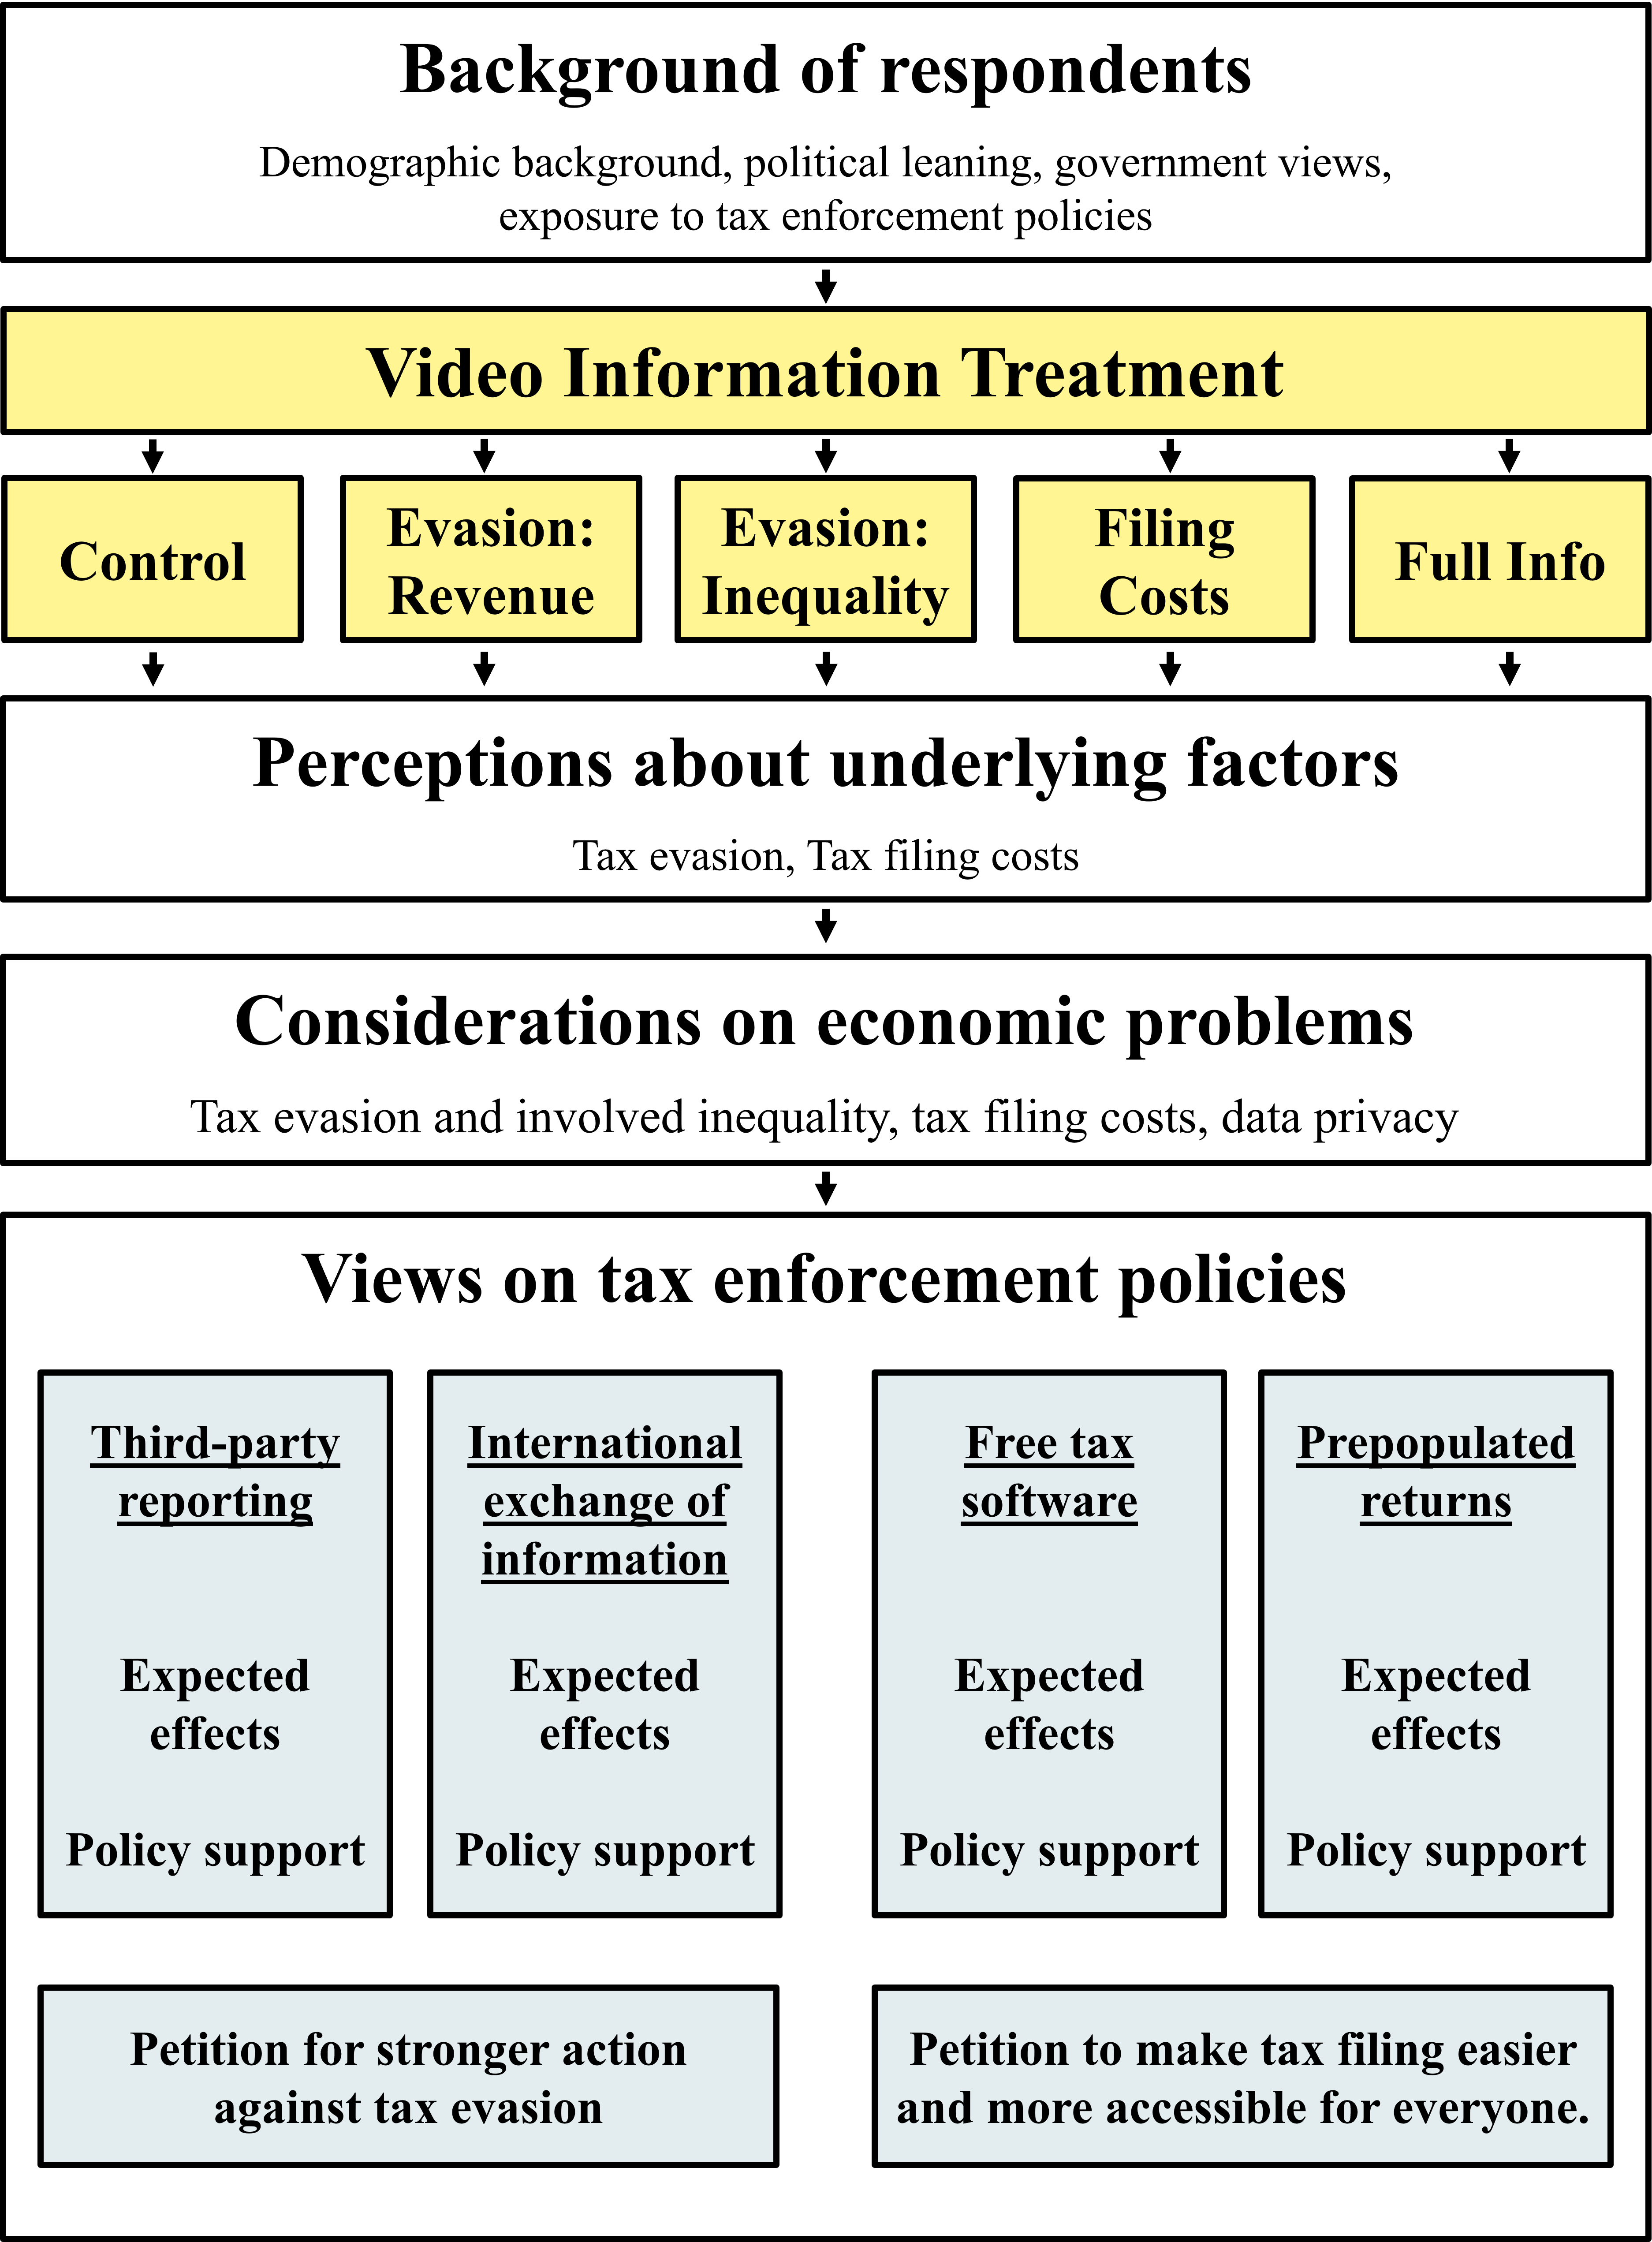
\includegraphics[width=1.05\linewidth]{Figures_Slides/Survey_Overview_Treatments.png}
  \end{column}
\end{columns}
\end{frame}

\begin{frame}
\label{frame:treatments}
  \centering
  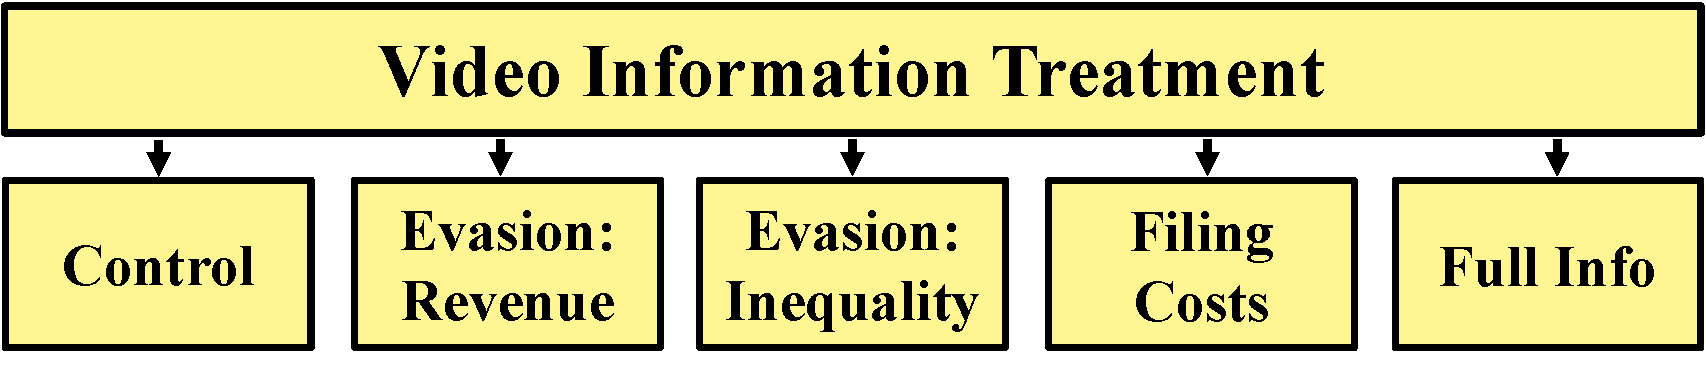
\includegraphics[width=0.7\textwidth]{Figures_Slides/Survey_Overview_Treatments_Focus.pdf}

  \vspace{1cm}
\centering
{\scriptsize
\begin{tabularx}{\textwidth}{*{4}{>{\centering\arraybackslash}X}}
  \textbf{Evasion: Revenue} & \textbf{Evasion: Inequality} & \textbf{Filing Costs} & \textbf{Full information} \\[0.5em]
  \textbf{1:48 min}  &
  \textbf{2:26 min}  &
  \textbf{2:56 min}  &
  \textbf{5:07 min} \\[0em]
  \begin{itemize}\item[$\Rightarrow$] Tax Evasion \& Government Revenue\end{itemize} &
  \begin{itemize}\item[$\Rightarrow$] Tax Evasion \& Government Revenue\end{itemize} &
   &
  \begin{itemize}\item[$\Rightarrow$] Tax Evasion \& Government Revenue\end{itemize} \\[-1em]
  &
  \begin{itemize}\item[$\Rightarrow$] Fairness \& Inequality\end{itemize} &
  &
  \begin{itemize}\item[$\Rightarrow$] Fairness \& Inequality\end{itemize} 
  \\[-1em]
&
&
  \begin{itemize}\item[$\Rightarrow$] Filing Costs \end{itemize} &
  \begin{itemize}\item[$\Rightarrow$] Filing Costs \end{itemize} \\
  \centering \hyperlink{frame:Evasionrevenue}{\beamergotobutton{Evasion: Revenue}}&
  \centering \hyperlink{frame:Evasioninequality}{\beamergotobutton{Evasion: Inequality}}&
  \centering \hyperlink{frame:Taxfiling}{\beamergotobutton{Filing Costs}}& 
  \centering \hyperlink{frame:Fullinfo}{\beamergotobutton{Full Info}}
\end{tabularx}
} \\

\end{frame}


\begin{frame}{Post Treatment}
\label{posttreatment}
\begin{columns}[T] % align columns at the top
  \begin{column}{0.45\textwidth} % left side for text
  \begin{itemize}
      \item Perception / Knowledge
      \begin{itemize}
          \item Level of tax evasion
          \item Level of tax filing costs
      \end{itemize} \vspace{0.25em}
      \item Considerations on underlying economic problems \hyperlink{Example:ConsiderationsEconomicProblems}{\beamergotobutton{Considerations}} \vspace{0.25em}
      \item Views on policies \vspace{0.25em} 
      \begin{itemize}
          \item Expected effects: \alert{focus on revenue, inequality, filing costs, data privacy} \hfill \hyperlink{Example:ExpectedEffects}{\beamergotobutton{Expected Effects}}\vspace{0.25em} \textit{}
          \item Policy support: general and conditional \hfill \hyperlink{Example:PolicySupport}{\beamergotobutton{Policy Support}}\vspace{0.25em} 
          \item Petition: helps to validate support
      \end{itemize}
  \end{itemize}
  \end{column}
  
  \begin{column}{0.45\textwidth} % right side for image
    \centering
     \vspace{-1em}     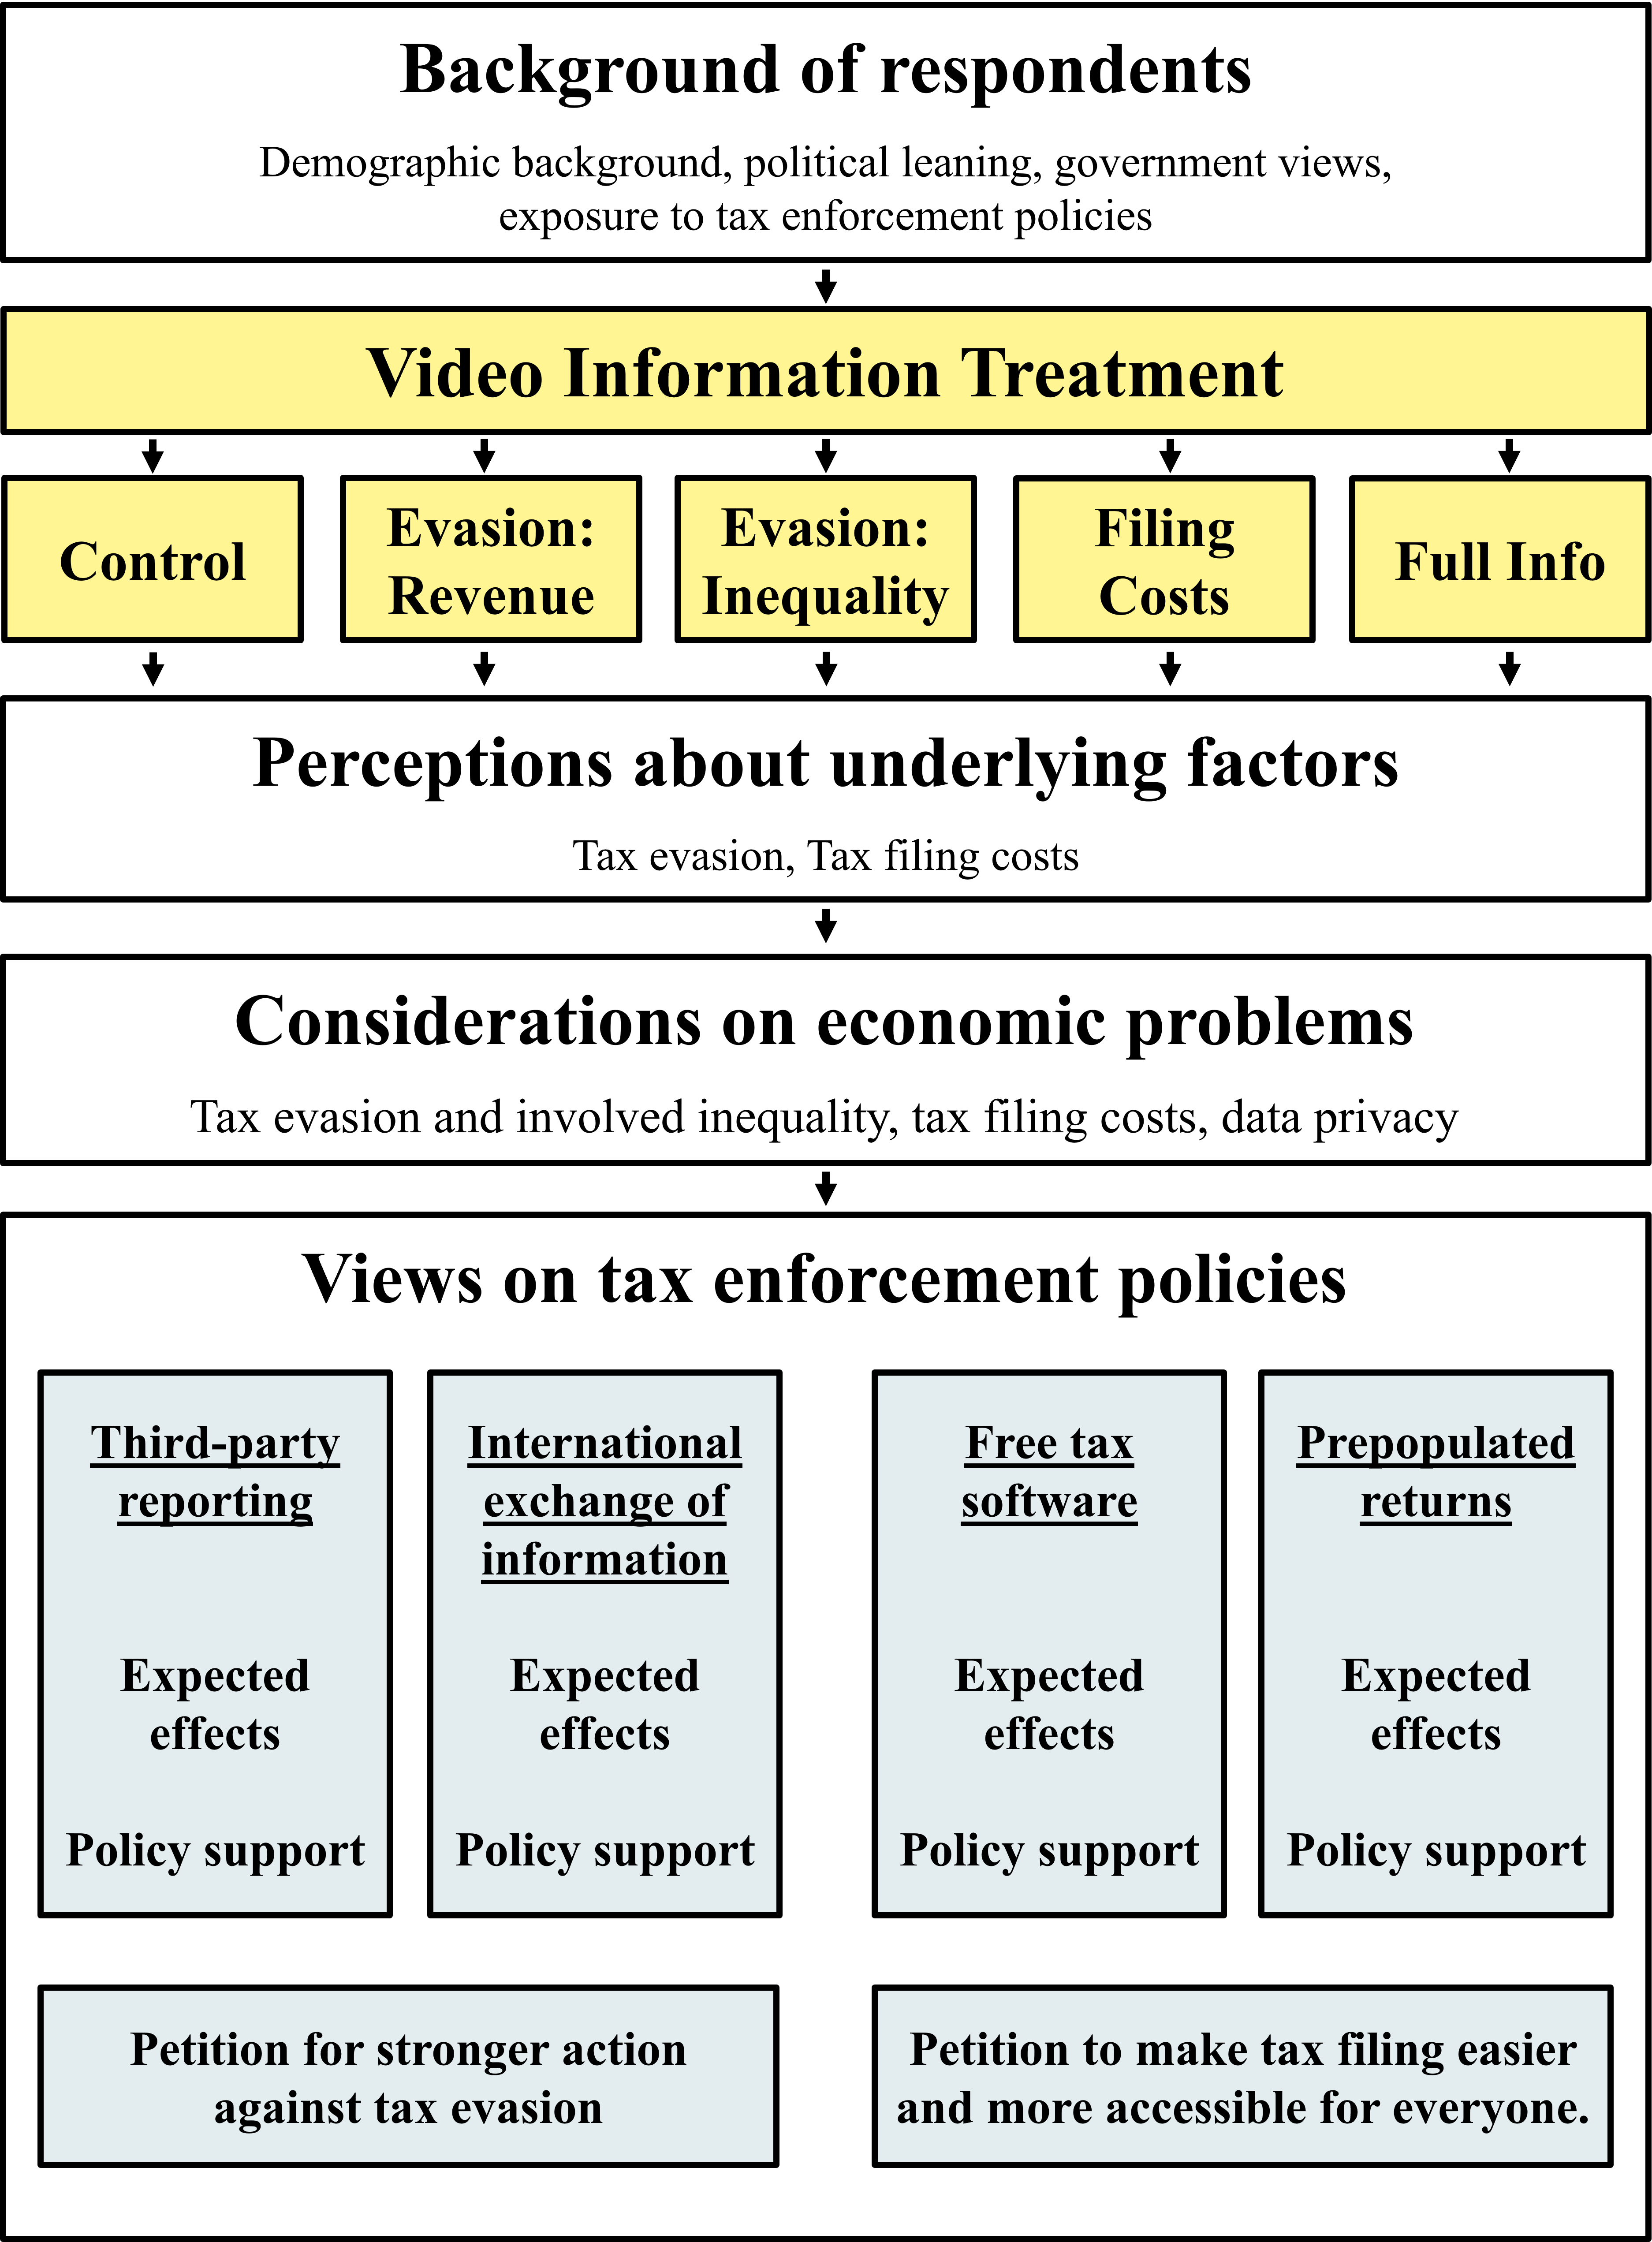
\includegraphics[width=1.05\linewidth]{Figures_Slides/Survey_Overview_Treatments.png}
  \end{column}
\end{columns}
\end{frame}


%\begin{frame}{Conclusion}
%\begin{itemize}
%\item Using a survey \alert{we explore peoples' attitudes and considerations towards information-sharing and free tax filing services.} 
%\begin{itemize}
%\item Towards more comprehensive third-party reporting and international automatic exchange of information.
%\item Towards free tax software and/or prepopulated tax returns.
%\end{itemize}
%\vspace{0.5em}
%\item We include questions to \alert{uncover important drivers of policy views.}
%\begin{itemize}
%    \item Perceptions, beliefs and important considerations 
%\end{itemize}
%\vspace{0.5em}
%\item To \alert{establish causal links} between reasoning and policy views, we \alert{experimentally show} people different educational \alert{videos}.
%\end{itemize}
%\end{frame}

\begin{frame}
\centering
\vfill

{\Huge \textbf{Thank you for listening!}} \\[1.5em]

{\Large Questions and feedback to:} \\[0.5em]
\texttt{tim.kircali@unisg.ch}

\vfill
\end{frame}

\appendix

\begin{frame}{Motivation: Tax Filing Costs}
\begin{columns} % align at top
  % Left column (text)
  \begin{column}{0.5\textwidth}
  \begin{itemize}
    \item US tax payers face high \alert{tax filing costs} and are urged to buy commercial tax software to file tax returns.
    \vspace{1em}
    \item \alert{Efforts to introduce free IRS software and prepopulated tax returns repeatedly blocked.} 
    \vspace{1em}
    \item Main arguments against government provided filing services are \alert{data privacy concerns and overreach of the federal government.}
  \end{itemize}
  \end{column}

  % Right column (figure)
  \begin{column}{0.5\textwidth}
  \begin{center}
    \fbox{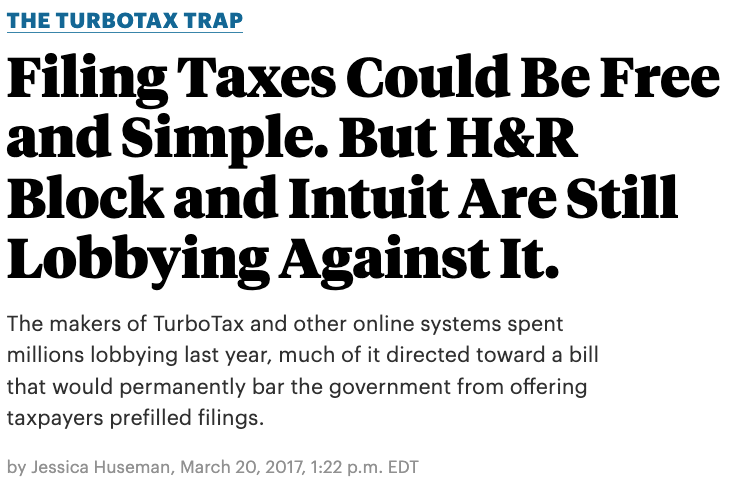
\includegraphics[width=0.9\linewidth]{Figures_Slides/Screenshot_News.png}} 

    \vspace{1.5em} % space between first and second

    \fbox{
\includegraphics[width=0.9\linewidth]{Figures_Slides/Article2.png}} 

    \vspace{0.2em} % space between second and third

    \fbox{
\includegraphics[width=0.9\linewidth]{Figures_Slides/Article_3_1.png}} 
\end{center}
  \end{column}
\end{columns}
\end{frame}


\begin{frame}{Motivation: Tax Evasion}
\begin{enumerate}
\centering
    \item \alert{Tax evasion} is a serious problem in many countries.
    \vspace{1em}
\end{enumerate}
    %\begin{itemize}
        %\item In the U.S. \$696B (15\%) taxes are not paid on time and \$606B (13\%) are never collected. \parencite{IRS_TaxGap_2022_Pub5869} 
    %\end{itemize}
    \begin{center}
        \fbox{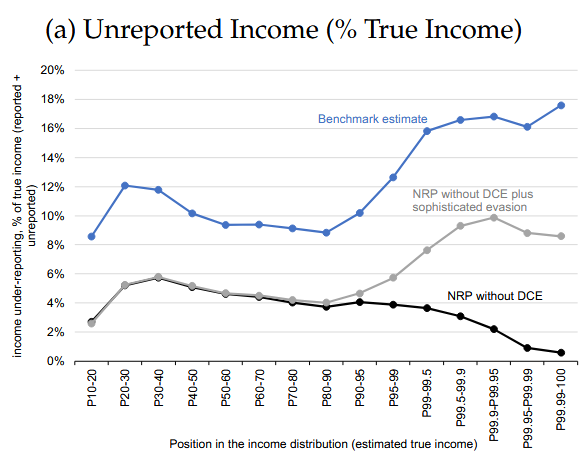
\includegraphics[width=0.45\linewidth]{Figures_Slides/Guyton.png}}
    \end{center}
    \vspace{-0.5em}
\begin{enumerate}
\centering
\setcounter{enumi}{1}
    \item Tax evasion is much \alert{more prevalent among the highest-income} earners. \parencite{guyton2021tax,alstadsaeter2019tax}
\end{enumerate}
\end{frame}

%\begin{frame}
%\frametitle{This Paper: What We Do}
%\begin{itemize}
%    \item Explores \alert{attitudes} and considerations \alert{towards information-sharing and tax filing service provision}.
%    \begin{itemize}
%        \item Towards more comprehensive third-party reporting and international automatic exchange of information. \\[0.2em]
%        \item Towards free tax software and/or prepopulated tax returns.
%    \end{itemize}
%    \vspace{1em} 
%    \item Leverages a \alert{large-scale survey to uncover considerations and beliefs} underlying these policy views.
%    \begin{itemize}
%        \item How, and why do they differ among respondents?
%    \end{itemize}
%    \vspace{1em} 
%    \item \alert{Experimental information} provision to establish \alert{causal} links between considerations and support for the policies.
%\end{itemize}
%\end{frame}

\begin{frame}
\frametitle{Related Literature}
\begin{enumerate}
    \item Measuring support for economic policies using survey experiments
\begin{itemize}
\scriptsize
    \item Tax policy: {\tiny\textcite{stantcheva2021understanding}} \\[0.1em]
    Tax simplicity and tax progressivity: {\tiny\textcite{tarroux2019value}} 
    %\item Designing information provision experiments: {\footnotesize\textcite{haaland2023designing}}\\[0.2em]  
    %Run surveys: {\footnotesize\textcite{stantcheva2023run}}.
\end{itemize}
\scriptsize
    \item[$\Rightarrow$] \alert{Measuring support for information exchange and tax filing services.}
\end{enumerate}
\begin{enumerate}
\setcounter{enumi}{1}
\item Tax evasion, tax enforcement and information reporting
\begin{itemize}
\scriptsize
    \item Third-party reporting: {\tiny \textcite{kleven2011unwilling}, \textcite{pomeranz2015no}, \textcite{kleven2016can}, \textcite{slemrod2017does}, \textcite{jensen2022employment}} \\[0.1em]
    Automatic exchange of information: {\tiny \textcite{baselgia2023compliance}, \textcite{boas2024taxing}} \\[0.1em]
    \item Distribution of tax evasion: {\tiny \textcite{johns2010distribution}, \textcite{alstadsaeter2019tax}, \textcite{guyton2021tax}}  
\end{itemize}
\scriptsize
\item[$\Rightarrow$] \alert{How do these documented facts shape policy support for information exchange?}
\vspace{0.2em} 
\end{enumerate}
\begin{enumerate}
\setcounter{enumi}{2}
\item Tax compliance costs and government's role to reduce them 
\begin{itemize}
\scriptsize
    \item Tax filing costs: {\tiny\textcite{blumenthal1992compliance}, \textcite{benzarti2020taxing}}  \\[0.1em]
    Non-filing: {\tiny\textcite{hauck2024optional}} \\[0.1em]
    Tax complexity: {\tiny\textcite{benzarti2024rising}, \textcite{tarroux2019value}}  \\[0.1em]
    \item Prepopulated tax returns: {\tiny\textcite{goodman2023automated}} \\[0.1em]
\end{itemize}
\scriptsize
\item[$\Rightarrow$] \alert{Analyse support for prepopulated tax returns and tax software (and its drivers).} 
\item[$\Rightarrow$] \alert{Explore the relation of support for tax filing services with support for information sharing.}
\end{enumerate}
\end{frame}


\section{Survey and Sample}

\begin{frame}{Recruitment and Screening}
\begin{columns}[T] % align columns at the top
  \begin{column}{0.45\textwidth} % left side for text
    \begin{itemize}
    \item U.S. residents aged 18 to 69 are recruited through a commercial survey company (e.g. Prolific / Bilendi)
    \vspace{1em} 
    \item \alert{Quota representativity} 
    \begin{itemize}
        \item Dimensions gender, age, region and education
    \end{itemize}
    \vspace{1em} 
    \item \alert{Avoid selection}
    \begin{itemize}
        \item Recruit without revealing topic / identity
    \end{itemize}
    \vspace{1em} 
    \item Embedded \alert{attention checks} for high-quality responses. 
    \end{itemize}
  \end{column}
  
  \begin{column}{0.45\textwidth} % right side for image
    \centering
    \vspace{-2em}
    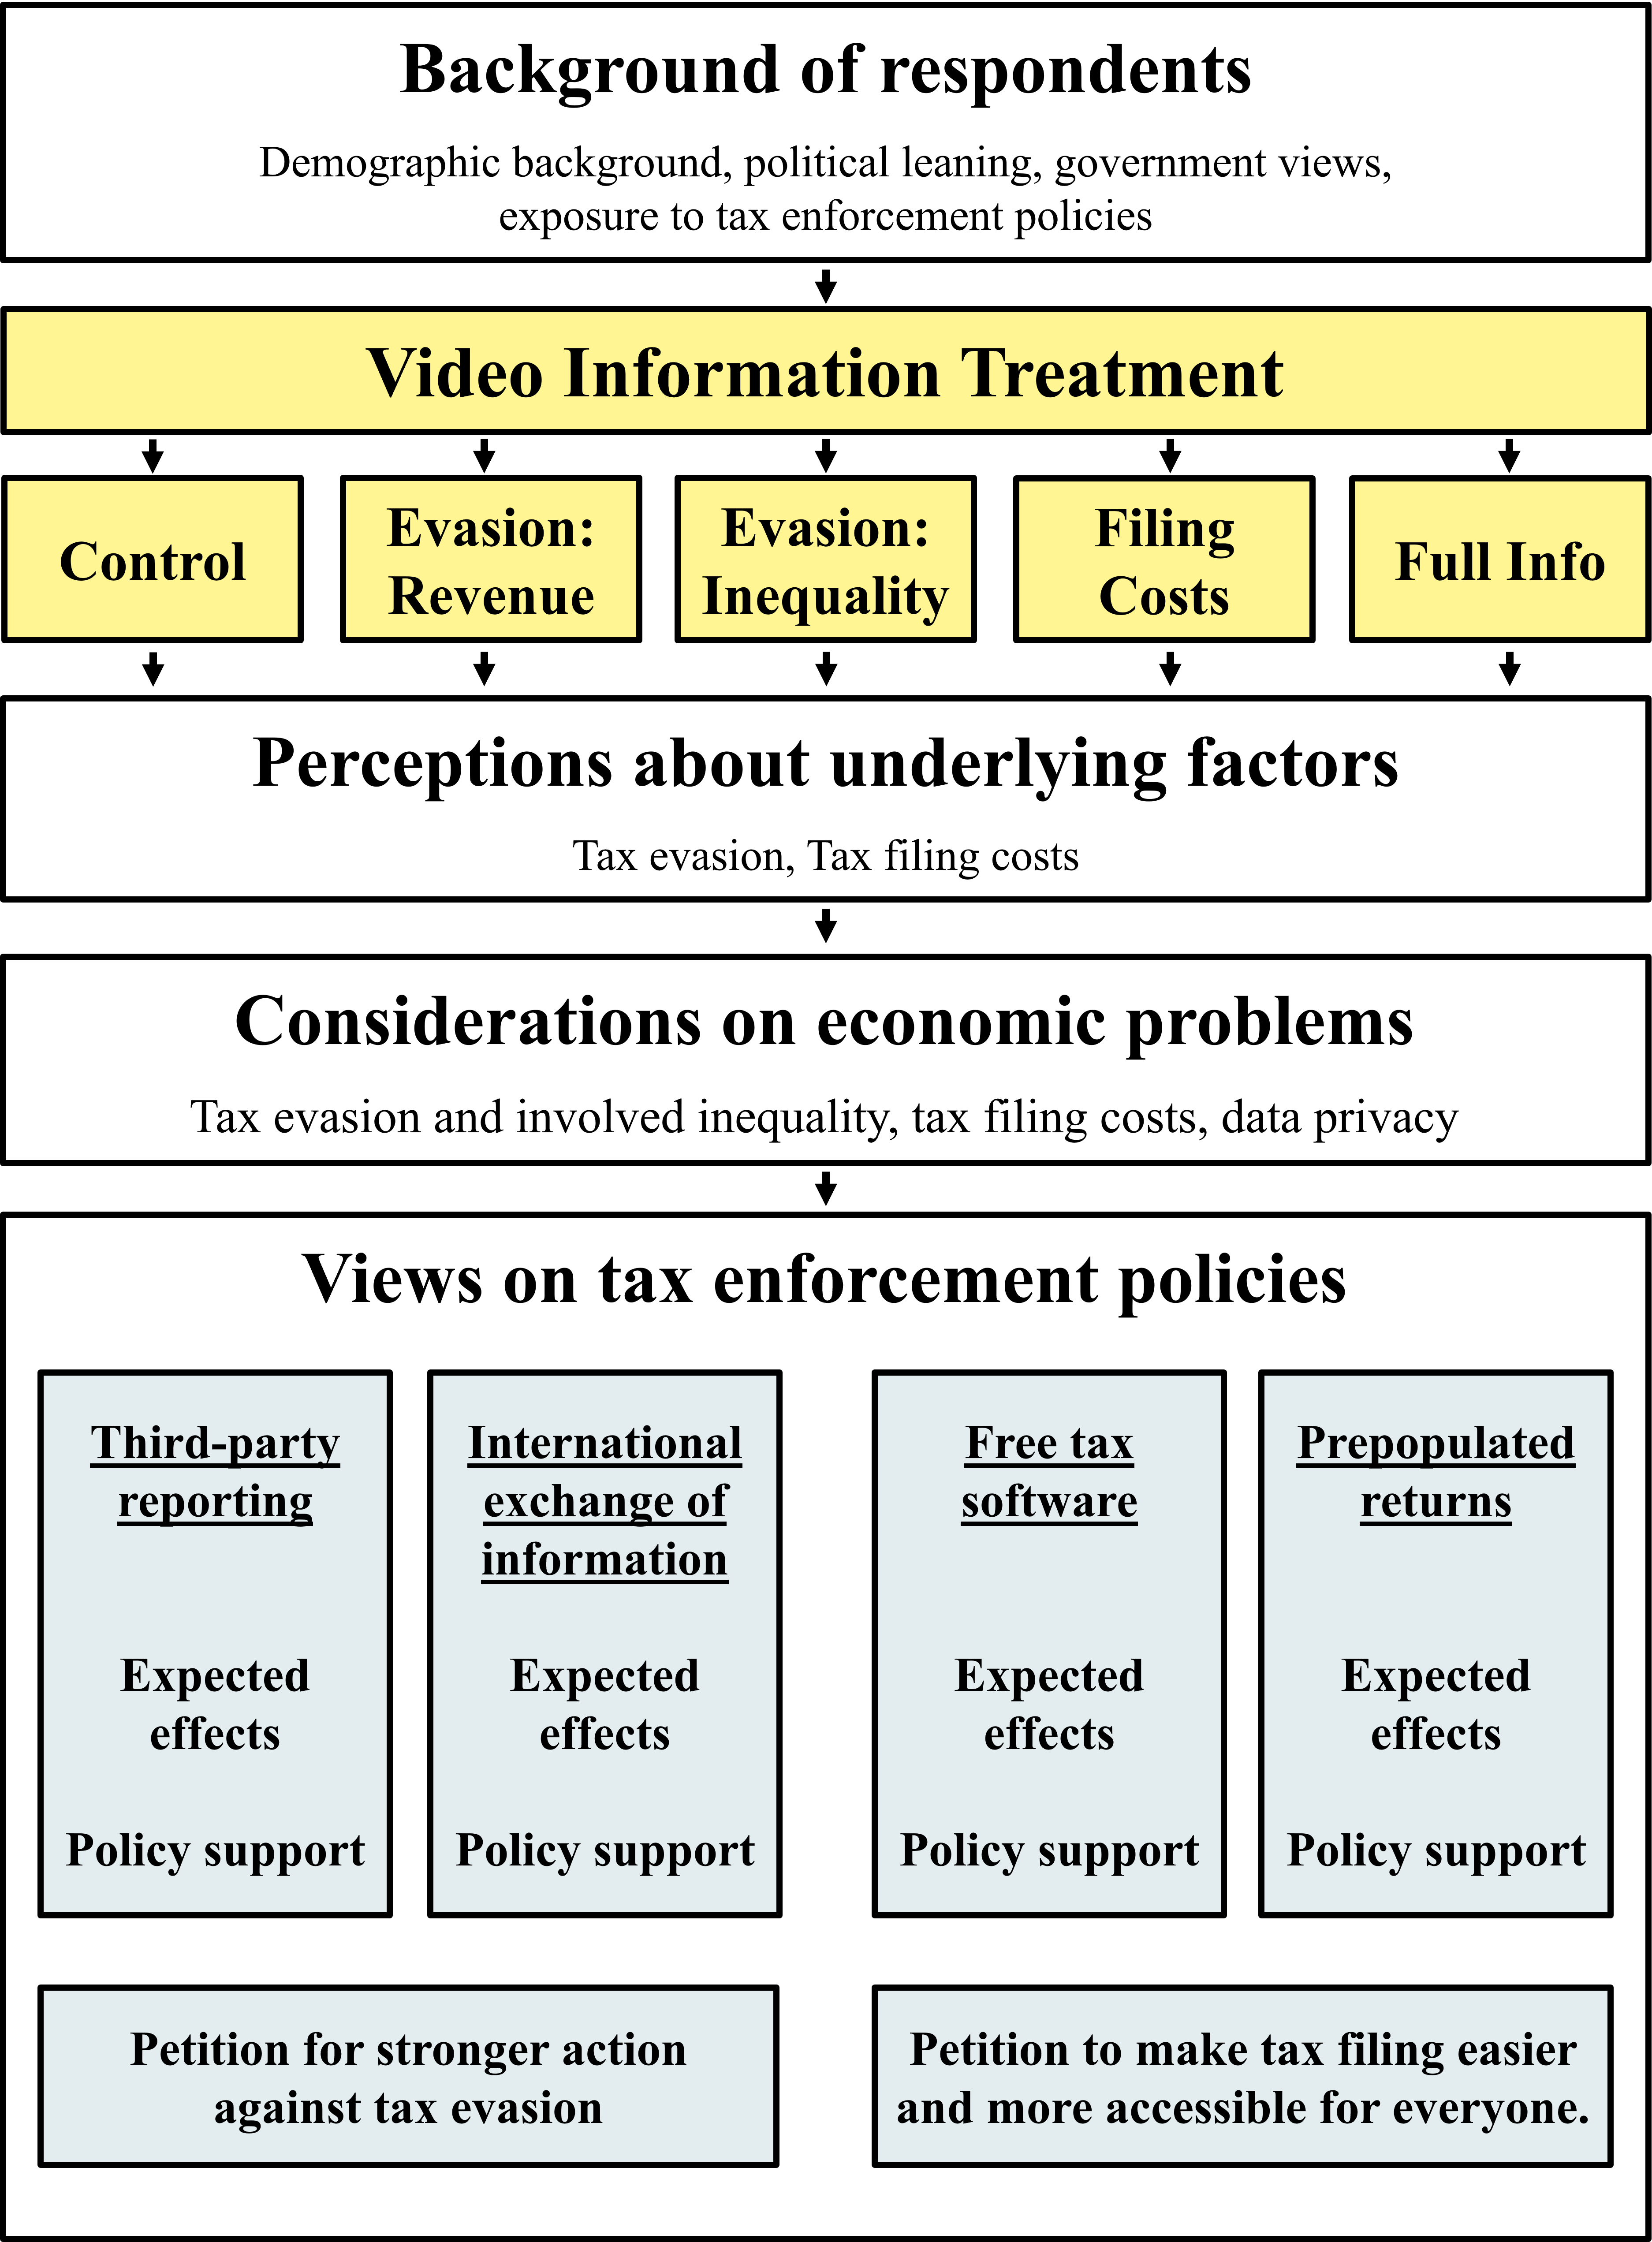
\includegraphics[width=1.05\linewidth]{Figures_Slides/Survey_Overview_Treatments.png}
  \end{column}
\end{columns}
\end{frame}

\begin{frame}[label=Personal_Exposure]{Background of Respondents}
\begin{columns}[T] % align columns at the top
  \begin{column}{0.45\textwidth} % left side for text
    \begin{itemize}
    \item Demographic background %(age, education, region, income, ethnicity, household composition) 
    \vspace{0.5em} 
    \item Political leaning
    \begin{itemize}
        \item Political affiliation
    \end{itemize}
    \vspace{0.5em} 
    \item Government views
    \begin{itemize}
        \item Trust
        \item Desired involvement
        \item Quality of services
    \end{itemize}
    \vspace{0.5em} 
    \item \alert{Exposure} to tax enforcement and tax administration
    \begin{itemize}
        \item Tax filing and tax software
        \item Filing mistakes and evasion
    \end{itemize}
    \end{itemize}
  \end{column}
  
  \begin{column}{0.45\textwidth} % right side for image
    \centering
     \vspace{-2em}
    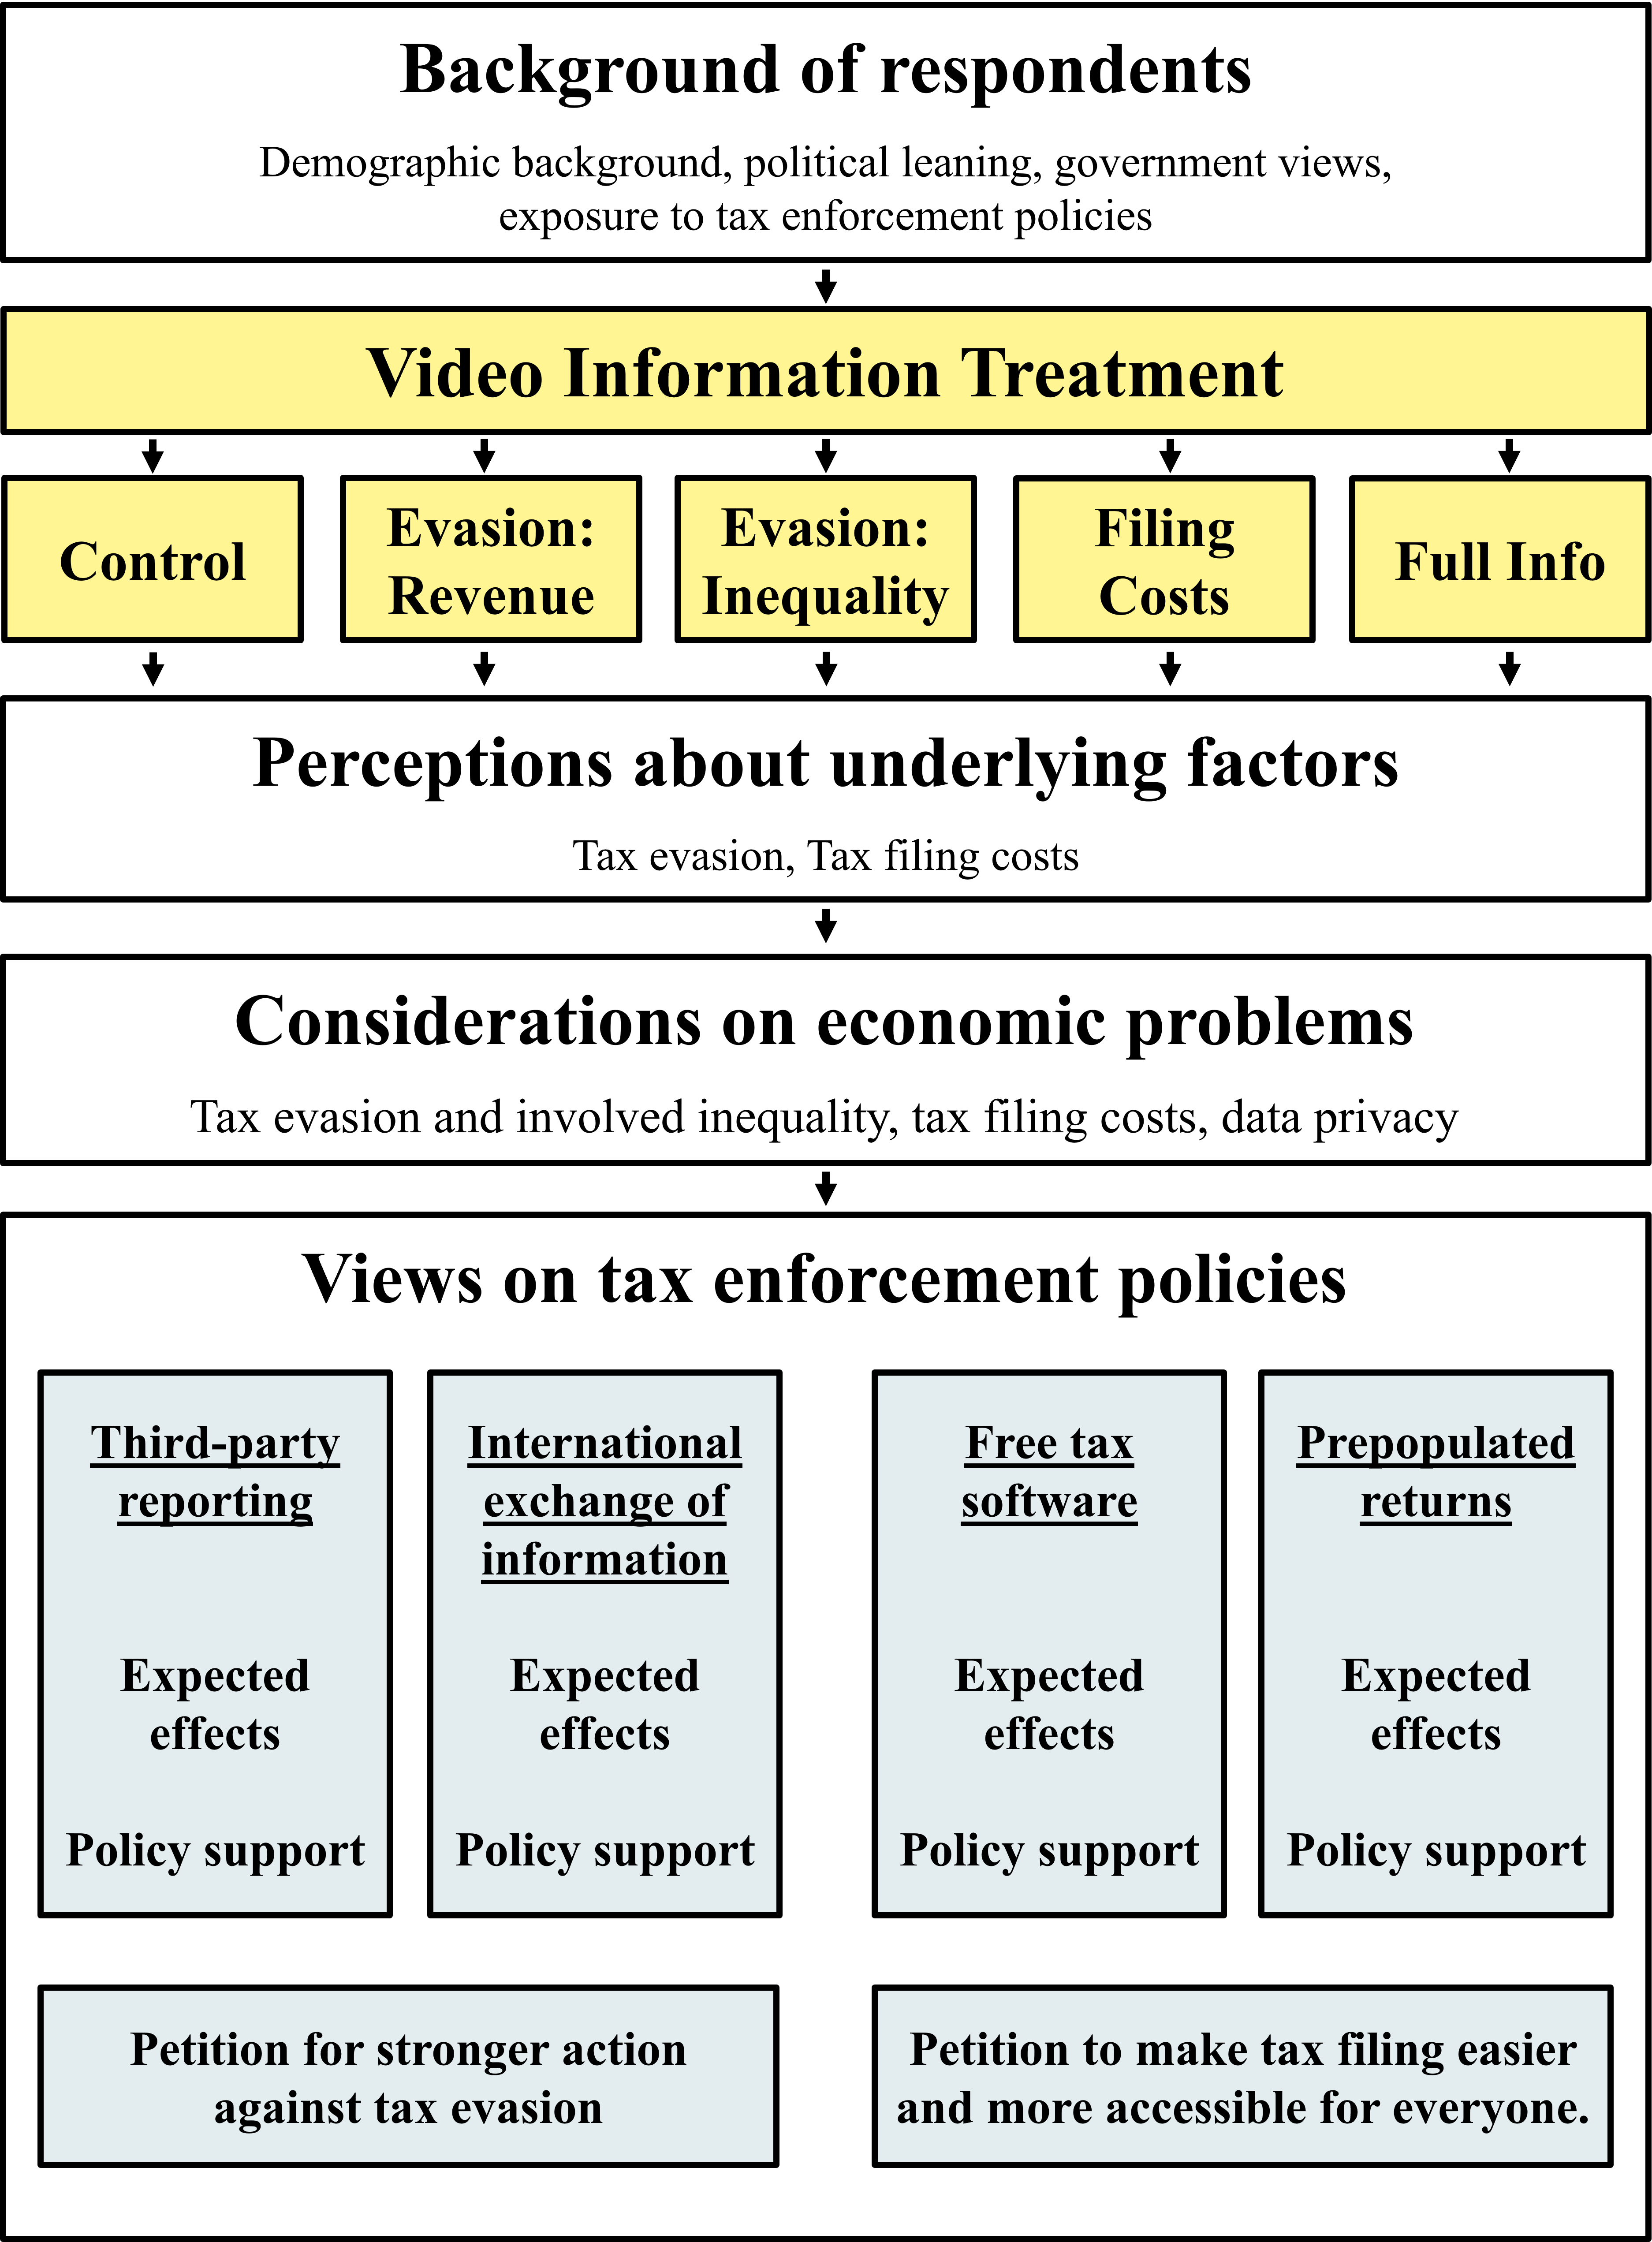
\includegraphics[width=1.05\linewidth]{Figures_Slides/Survey_Overview_Treatments.png}
  \end{column}
\end{columns}
\end{frame}

%\begin{frame}{Video Information Treatments}
%\begin{columns}[T] % align columns at the top
%  \begin{column}{0.45\textwidth} % left side for text
%    \begin{itemize}
%    \vspace{1em} 
%    \item Educational \alert{information videos}
%    \begin{itemize}
%        \item Audio
%        \item Subtitles
%        \item Animated
%    \end{itemize}
%    \vspace{1.5em} 
%    \item Close \alert{link to important underlying concerns} 
%    \begin{itemize}
%        \item Tax evasion \& revenue
%        \item Fairness \& inequality
%        \item Tax filing costs
%    \end{itemize}
%    \end{itemize}
%  \end{column}
%  
%  \begin{column}{0.45\textwidth} % right side for image
%    \centering
%     \vspace{-2em}     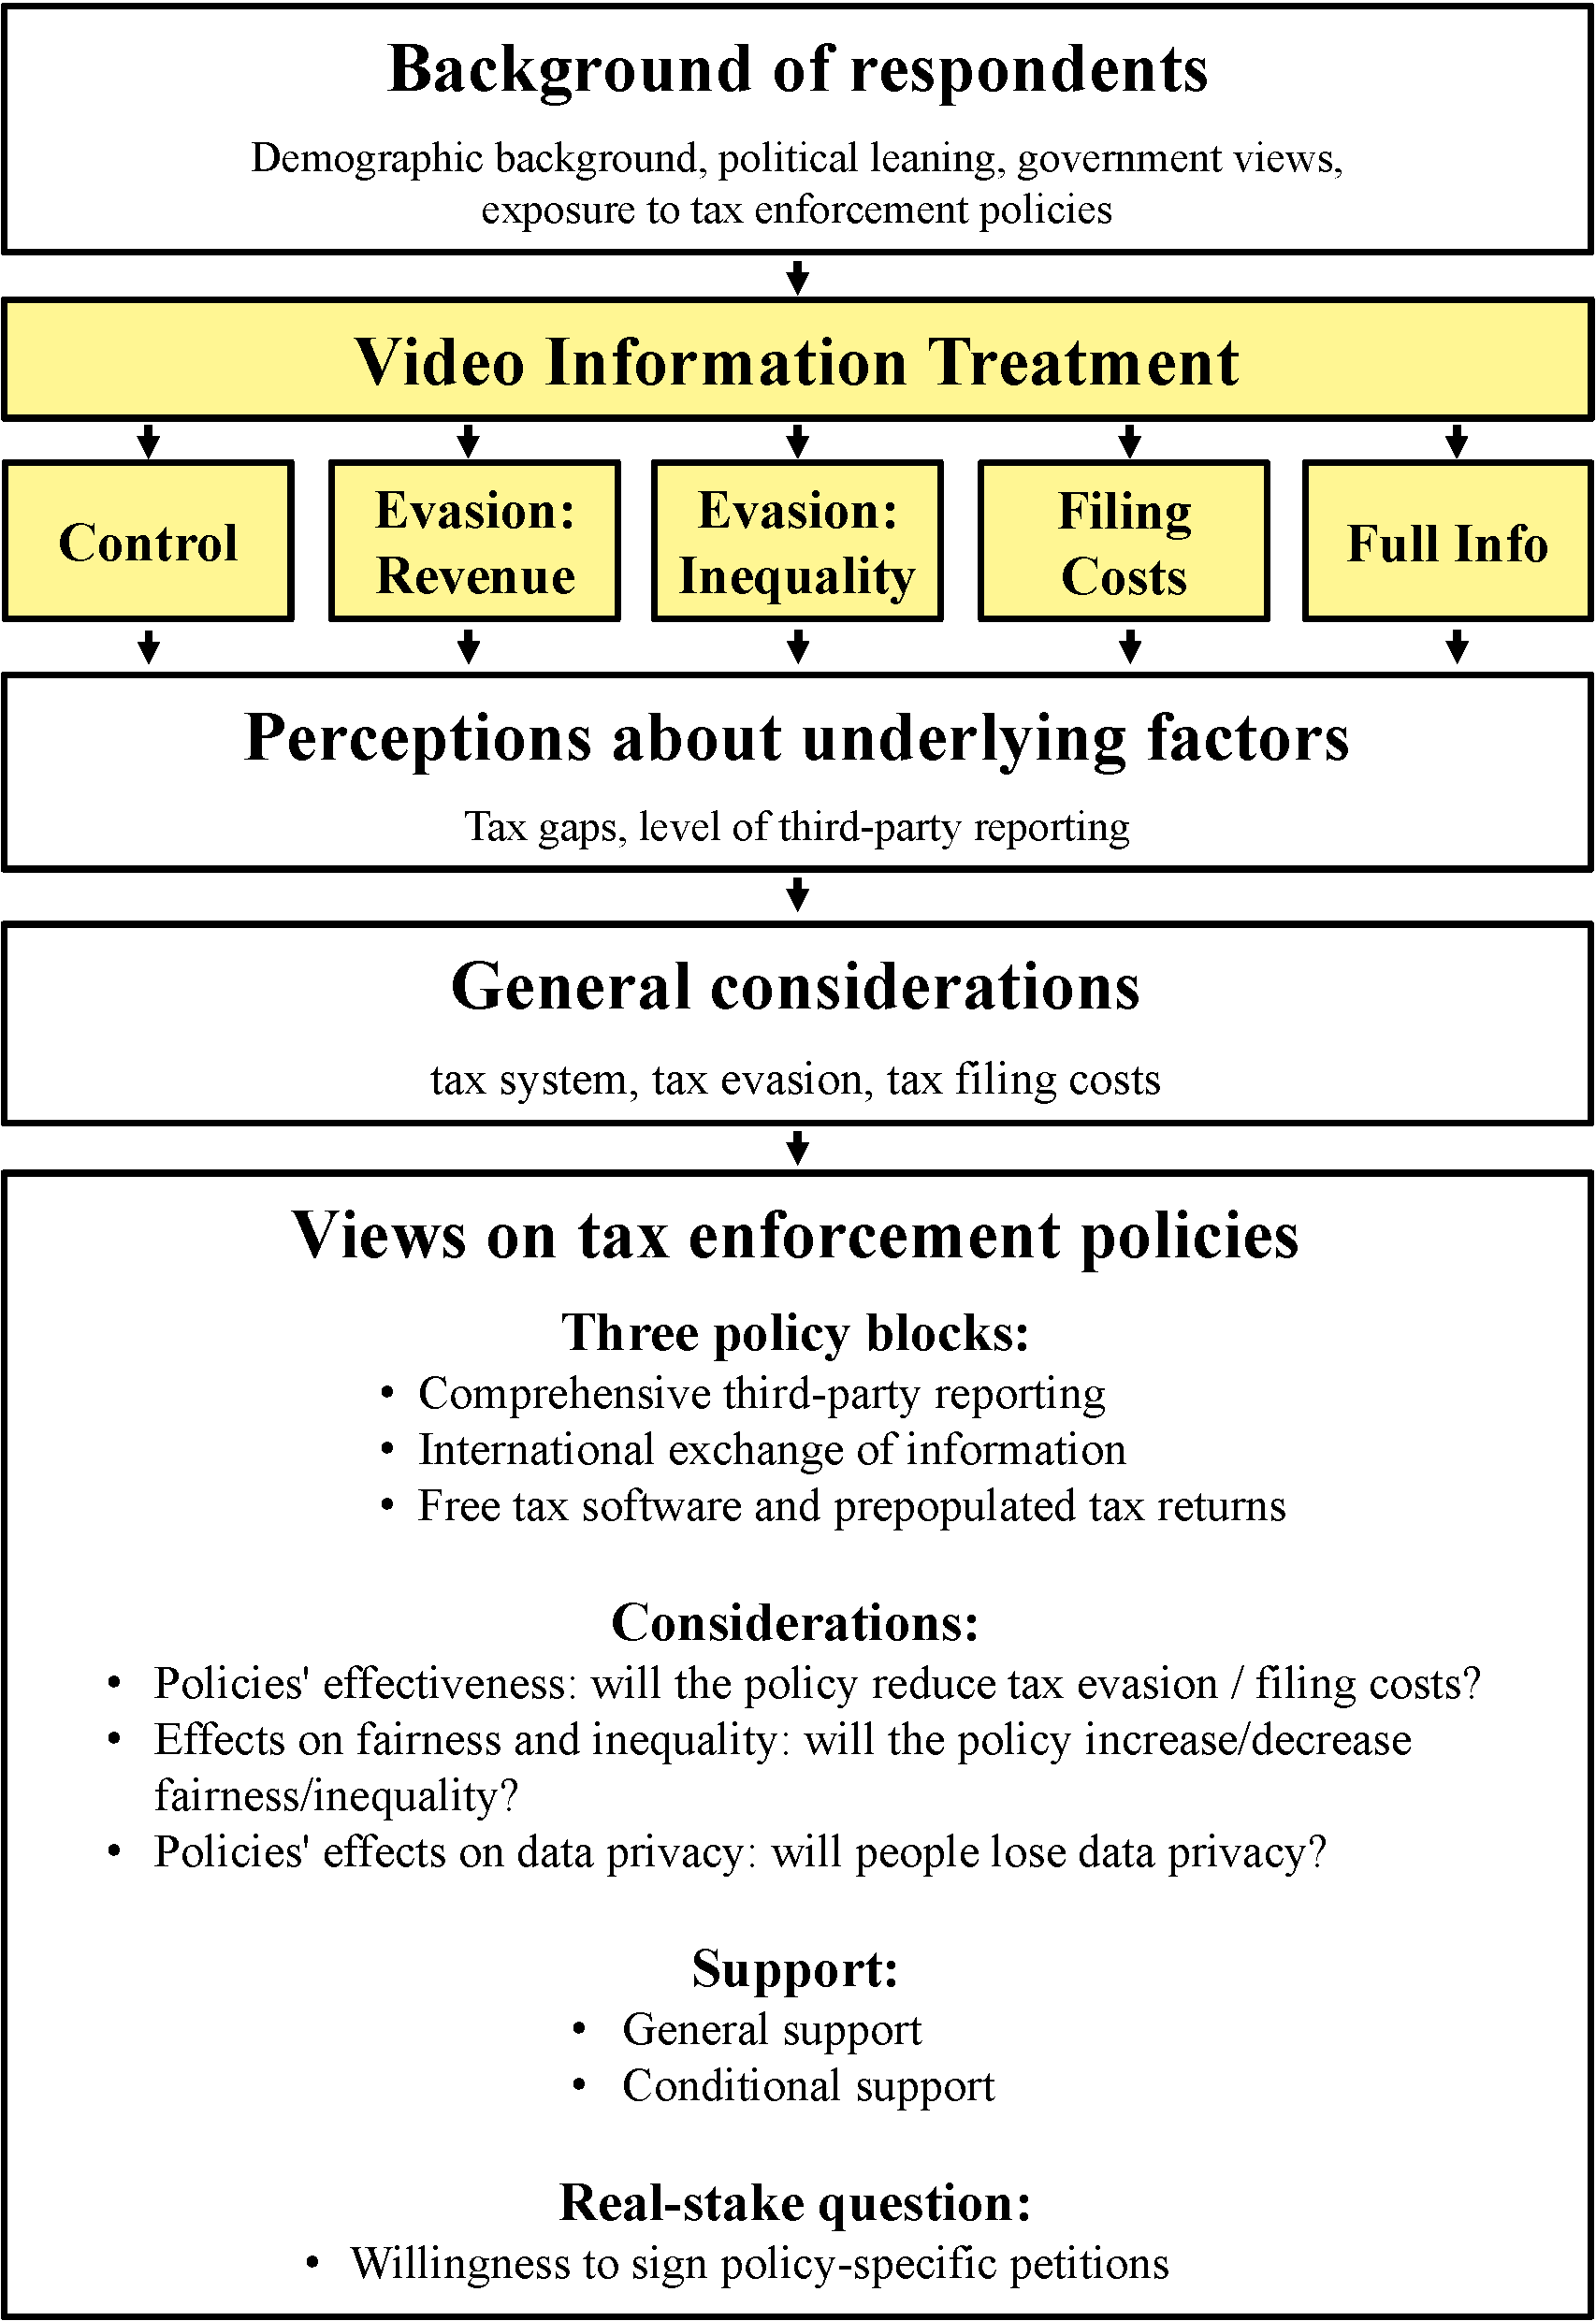
\includegraphics[width=1.05\linewidth]{Figures_Slides/Survey_Overview_Treatments.pdf}
%  \end{column}
%\end{columns}
%\end{frame}

%\begin{frame}{Video Information Treatments}
%\begin{columns}[T] % align columns at the top
%  \begin{column}{0.45\textwidth} % left side for text
%    \begin{itemize}
%    \vspace{1em} 
%    \item Educational \alert{information videos}
%    \begin{itemize}
%        \item Audio
%        \item Subtitles
%        \item Animated
%    \end{itemize}
%    \vspace{1.5em} 
%    \item Close \alert{link to important underlying concerns} 
%    \begin{itemize}
%        \item Tax evasion \& revenue
%        \item Fairness \& inequality
%        \item Tax filing costs
%    \end{itemize}
%    \end{itemize}
%  \end{column}
%  
%  \begin{column}{0.45\textwidth} % right side for image
%    %\vspace{0.3cm}
%    \centering
%    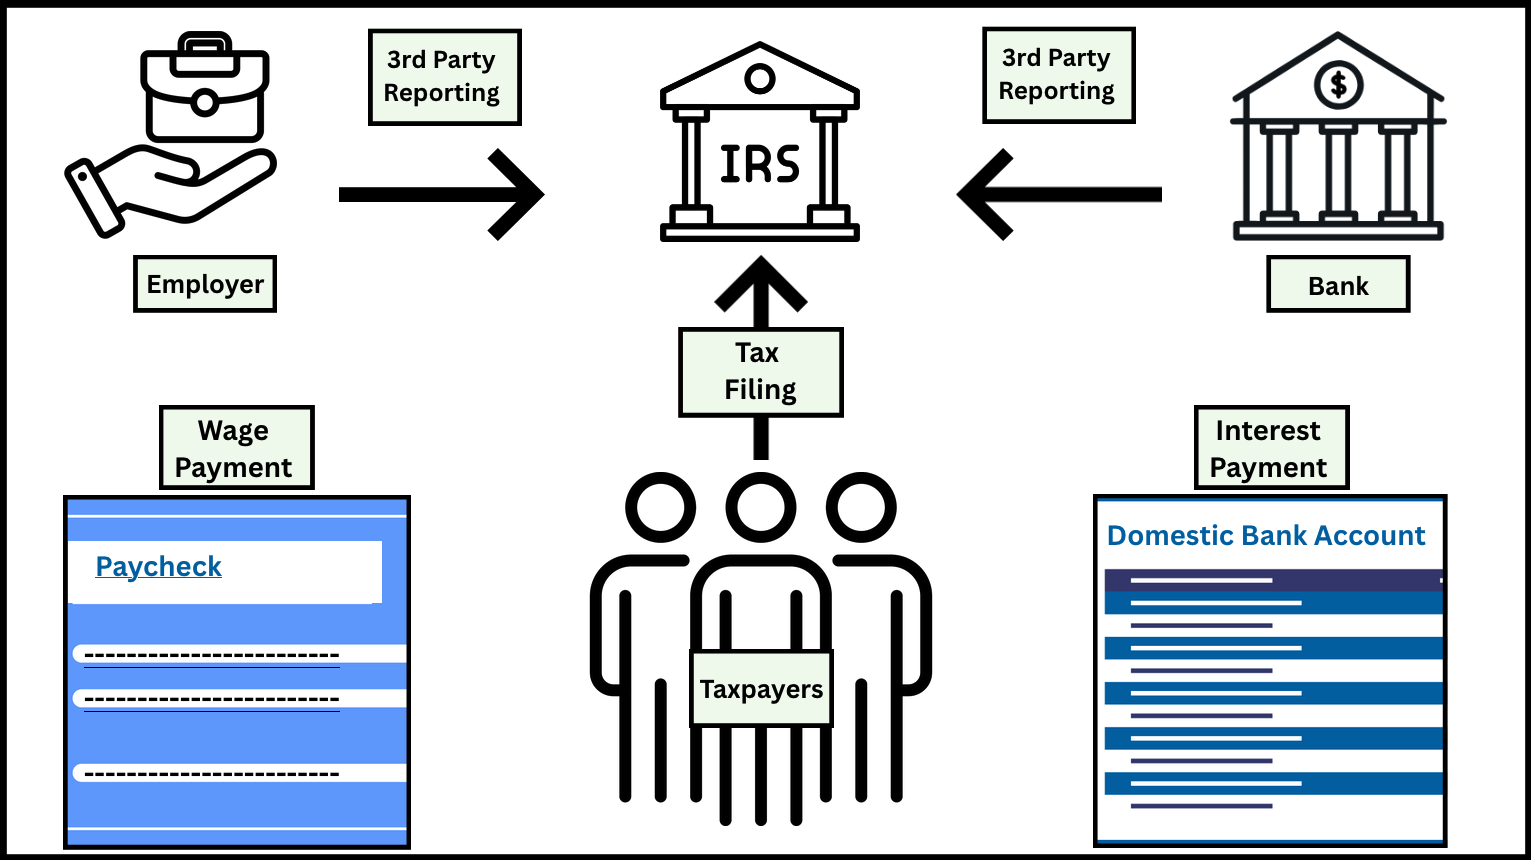
\includegraphics[width=0.95\linewidth]{Figures_Slides/Screenshot_3.png}\\[0.5cm]
%    %\vspace*{1cm}
%    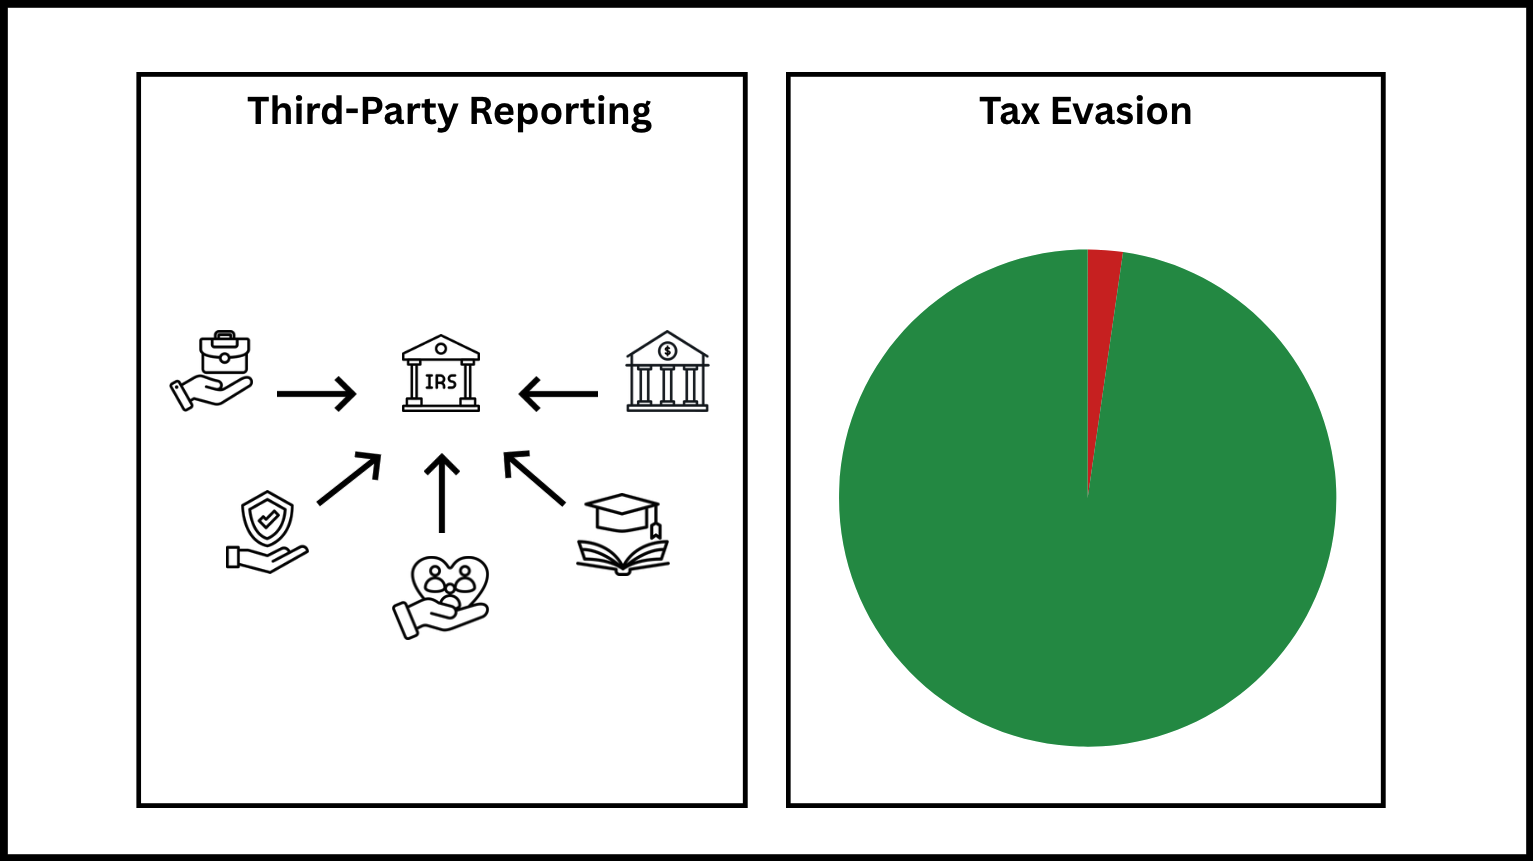
\includegraphics[width=0.95\linewidth]{Figures_Slides/Screenshot_2.png}
%  \end{column}
%\end{columns}
%\end{frame}
\begin{frame}{Evasion: Revenue}
\label{frame:Evasionrevenue}
\begin{columns}[T] % align columns at the top
  \begin{column}{0.45\textwidth} % left side for text
    \begin{itemize}
    \item Information about economic problem
    \begin{itemize}
    \vspace{0.25em}
        \item \alert{Extent} of tax evasion\footnote{\cite{IRS_TaxGap_2022_Pub5869}}
    \end{itemize}
    \vspace{2.5em} 
    \item Information about policy
    \begin{itemize}
    \vspace{0.25em}
        \item Third-party reporting \& IEoI \alert{reduces tax evasion}\footnote{ \cite{kleven2011unwilling,pomeranz2015no,kleven2016can,slemrod2017does,jensen2022employment,baselgia2023compliance,boas2024taxing}}
        \vspace{4.5em}
    \end{itemize}
    \end{itemize}
  \end{column}
  
  \begin{column}{0.45\textwidth} % right side for image
    %\vspace{0.3cm}
    \centering
    \vspace{-0.5em}
    \fbox{%
  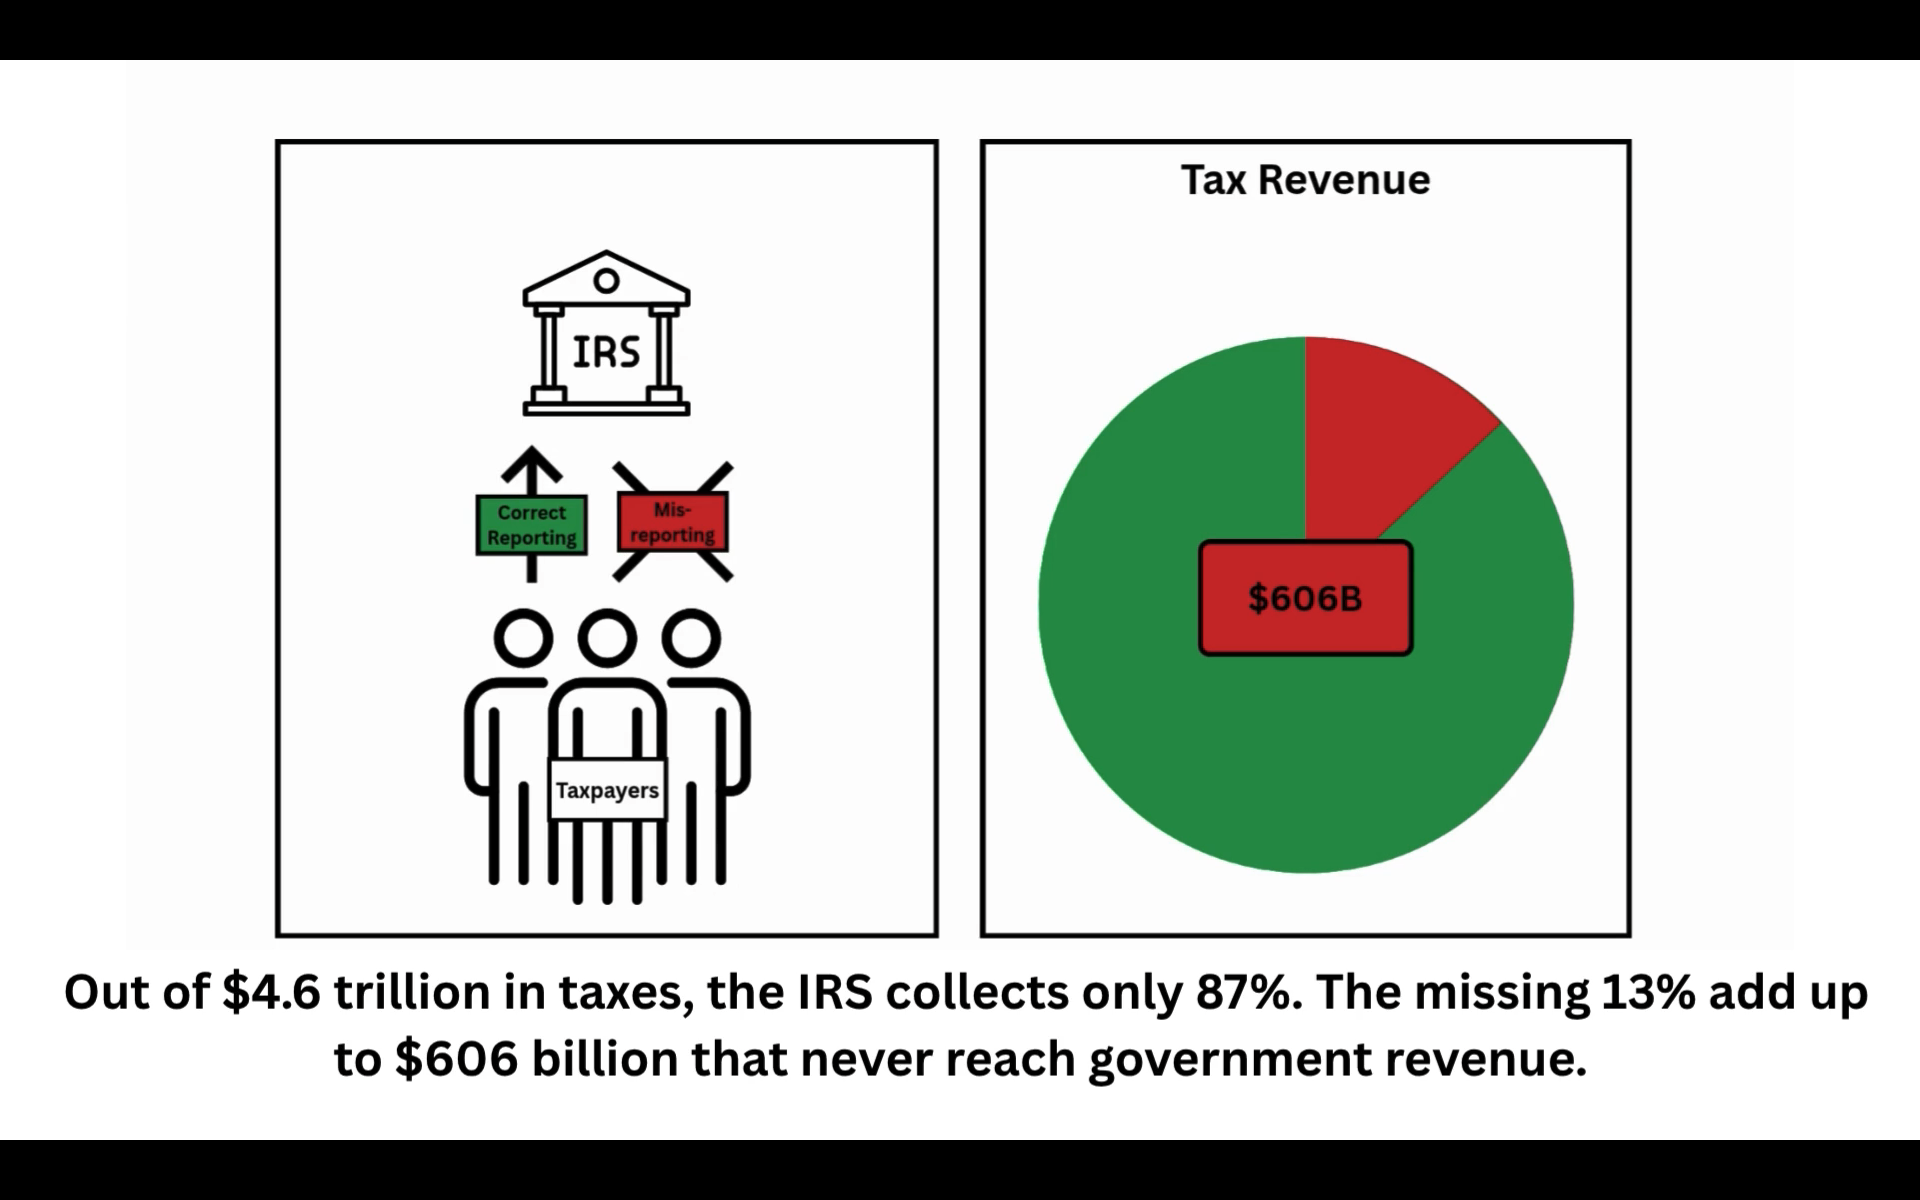
\includegraphics[width=\linewidth, trim={0.5cm 2.5cm 0.5cm 2.5cm}, clip]{Figures_Slides/Revenue_1.png}%
}\\[0.5cm]
    %\vspace*{1cm}
\fbox{%
  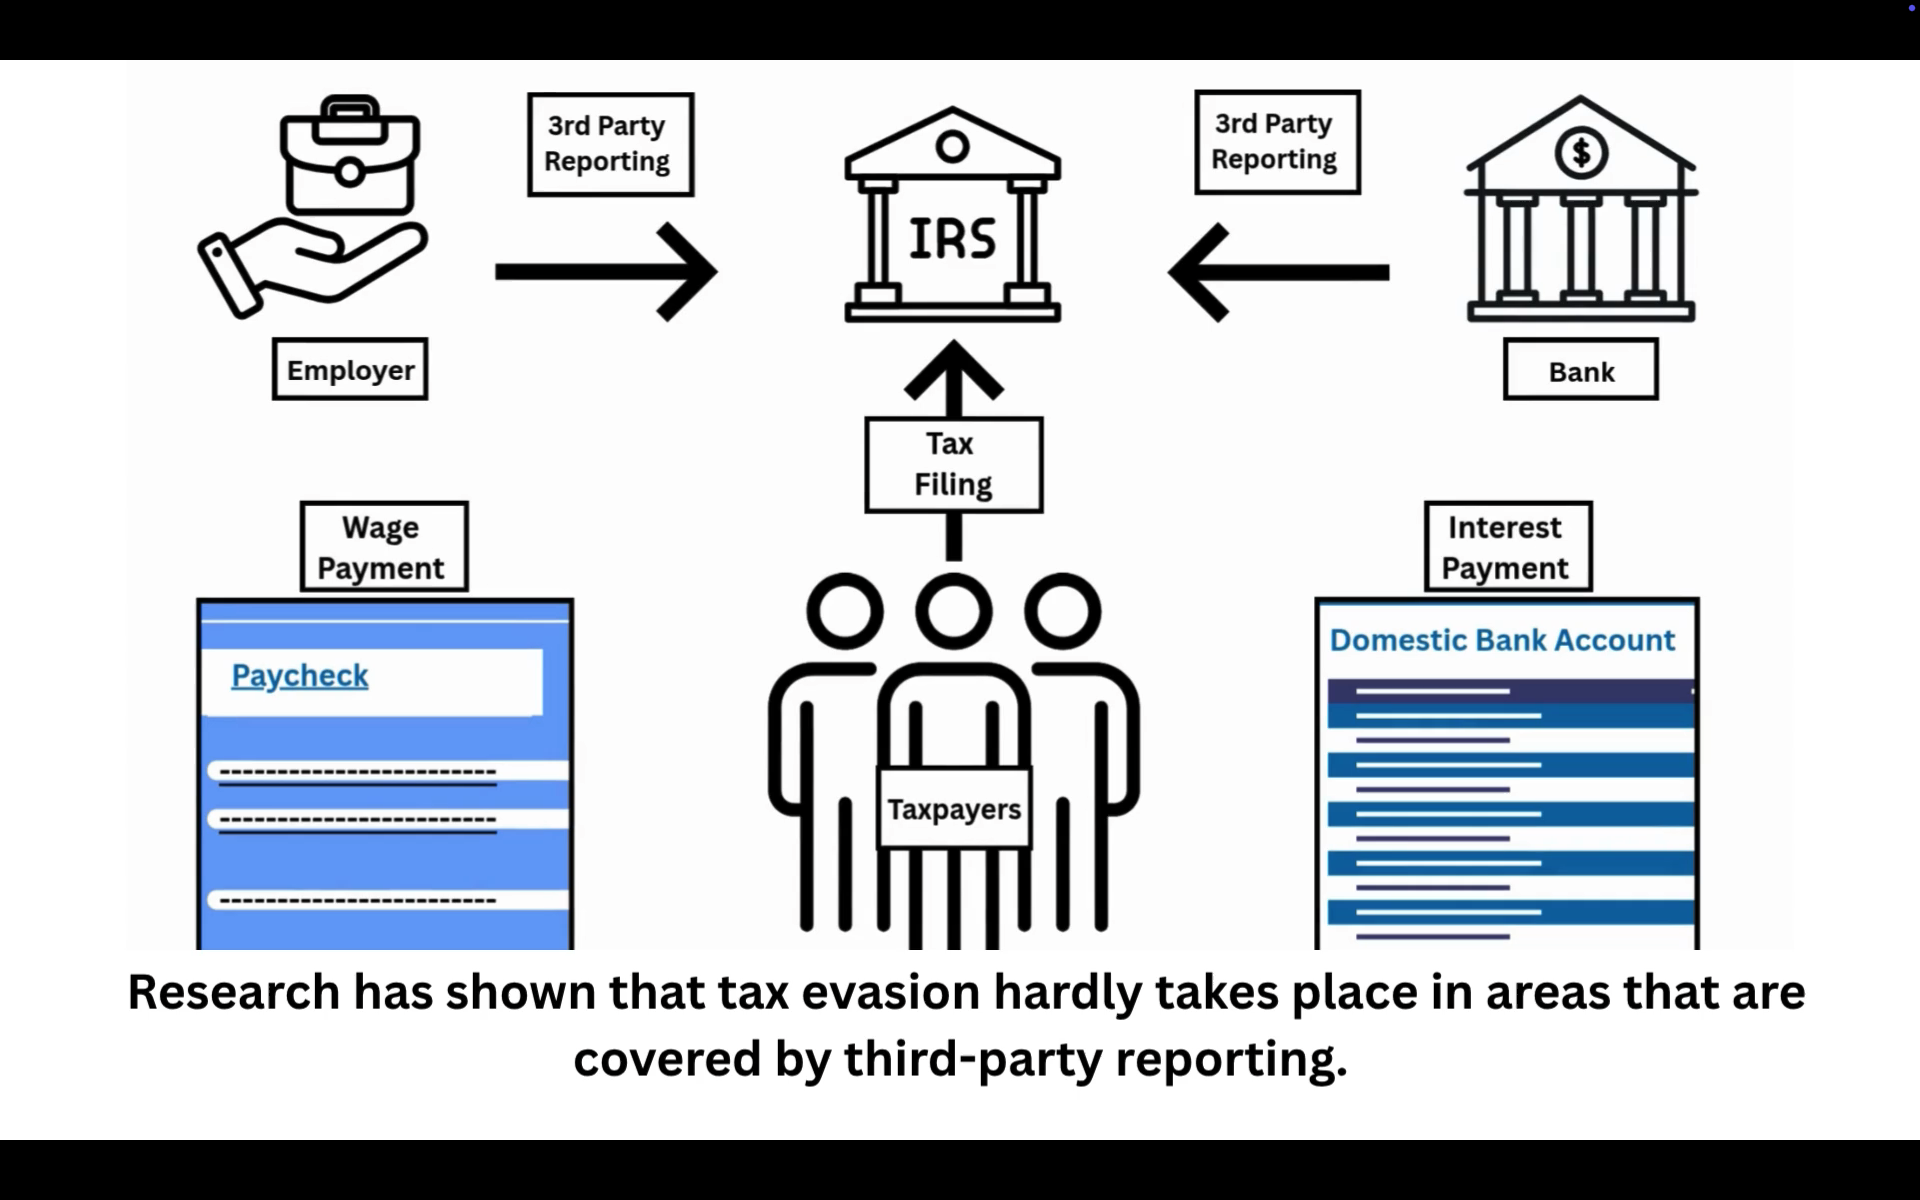
\includegraphics[width=\linewidth, trim={0.5cm 2.5cm 0.5cm 2.5cm}, clip]{Figures_Slides/Revenue_2.png}%
}\\[0.5cm]
\hfill \hyperlink{frame:treatments}{\beamergotobutton{Back}}
  \end{column}
\end{columns}
\end{frame}

\begin{frame}{Evasion: Inequality}
\label{frame:Evasioninequality}
\begin{columns}[T] % align columns at the top
  \begin{column}{0.45\textwidth} % left side for text
    \begin{itemize}
    \item Information about economic problem
    \begin{itemize}
    \vspace{0.25em}
        \item \alert{Extent} of tax evasion\footnote{\cite{IRS_TaxGap_2022_Pub5869}}
        \vspace{0.25em}
        \item \alert{Distribution} of tax evasion\footnote{\cite{guyton2021tax}}
    \end{itemize}
    \vspace{1.5em} 
    \item Information about policy
    \begin{itemize}
        \vspace{0.25em} 
        \item Third-party reporting \& IEoI \alert{reduces tax evasion}\footnote{ \cite{kleven2011unwilling,pomeranz2015no,kleven2016can,slemrod2017does,jensen2022employment,baselgia2023compliance,boas2024taxing}}
        \vspace{2.5em}
    \end{itemize}
    \end{itemize}
  \end{column}
  
  \begin{column}{0.45\textwidth} % right side for image
    %\vspace{0.3cm}
    \centering
    \vspace{-0.5em}
    \fbox{%
  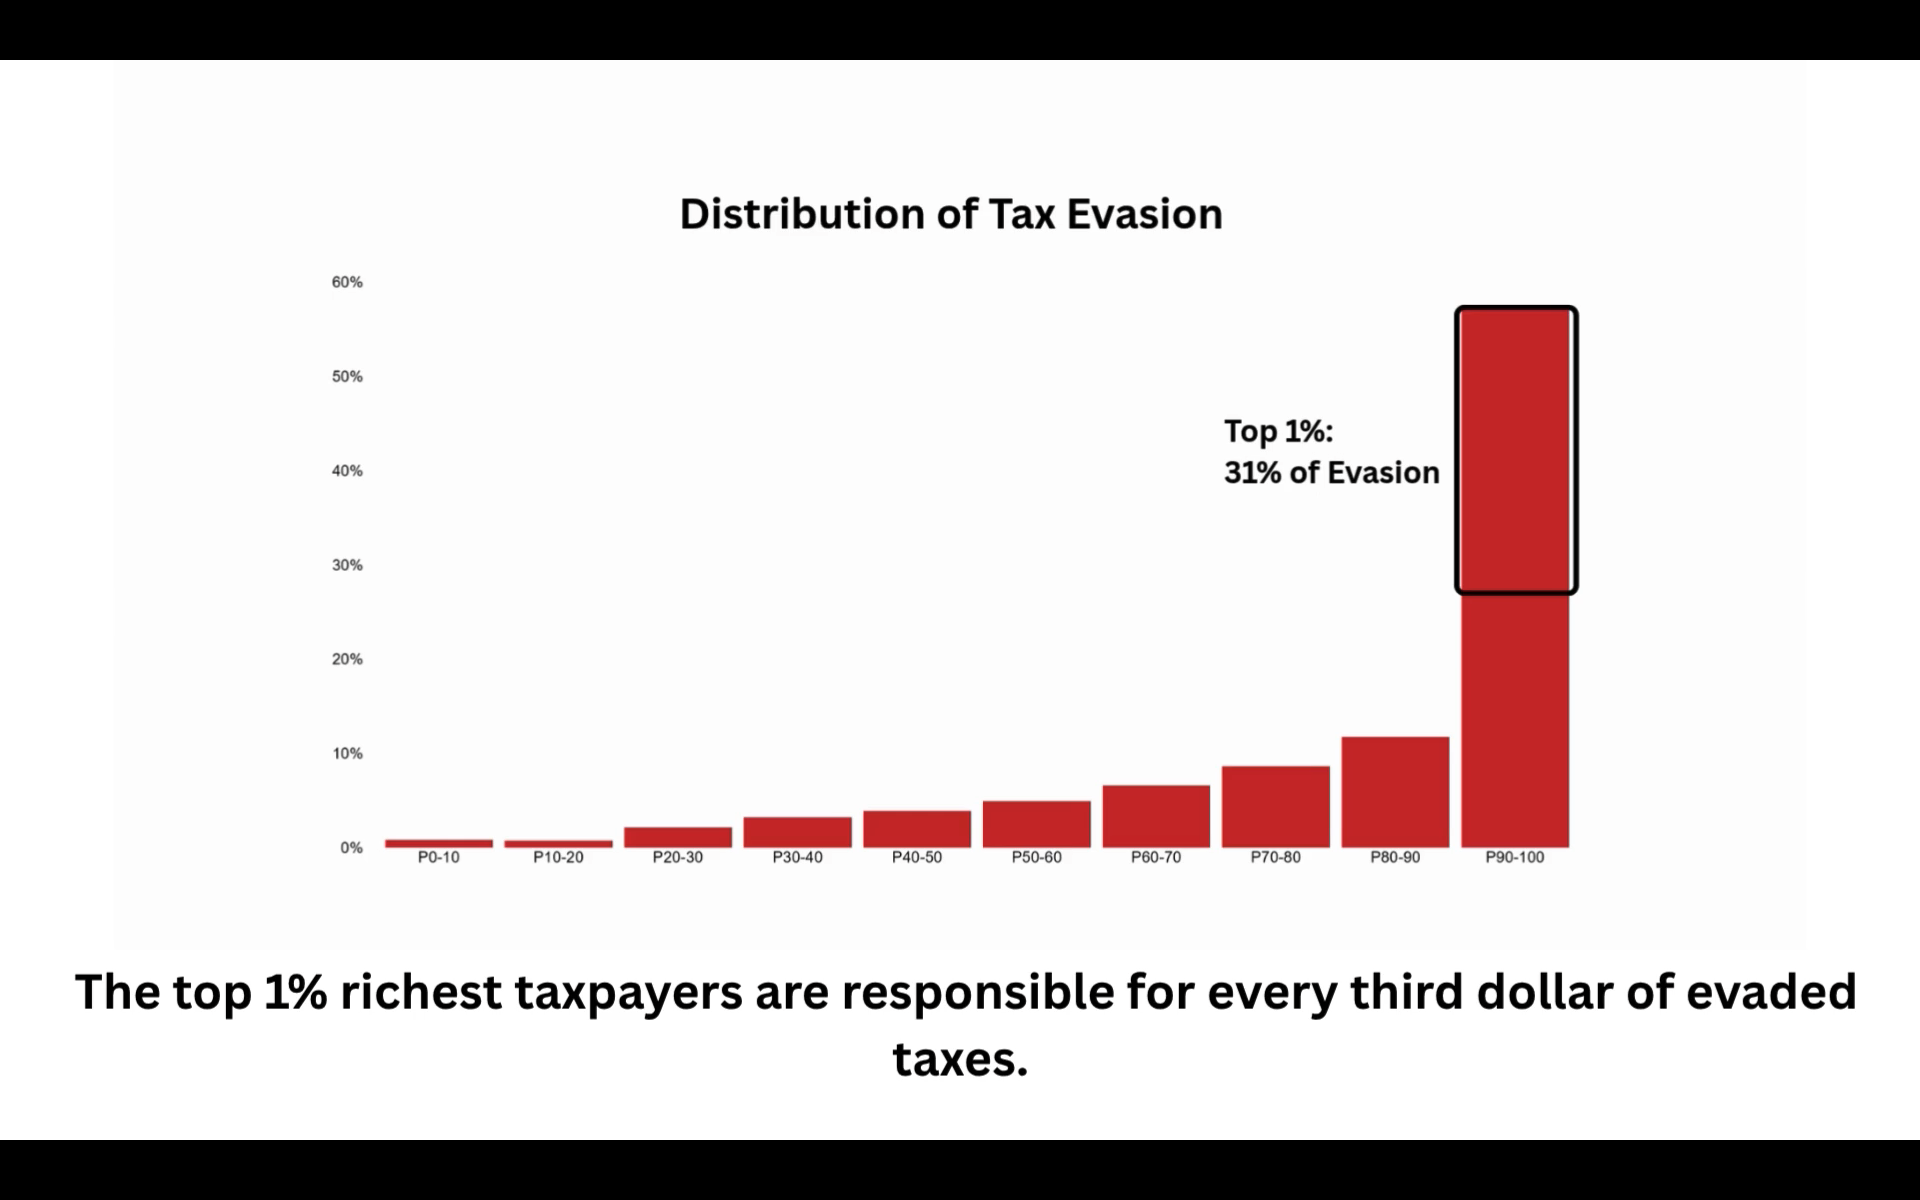
\includegraphics[width=\linewidth, trim={0.5cm 2.5cm 0.5cm 2.5cm}, clip]{Figures_Slides/Inequality_1.png}%
}\\[0.5cm]
    %\vspace*{1cm}
\fbox{%
  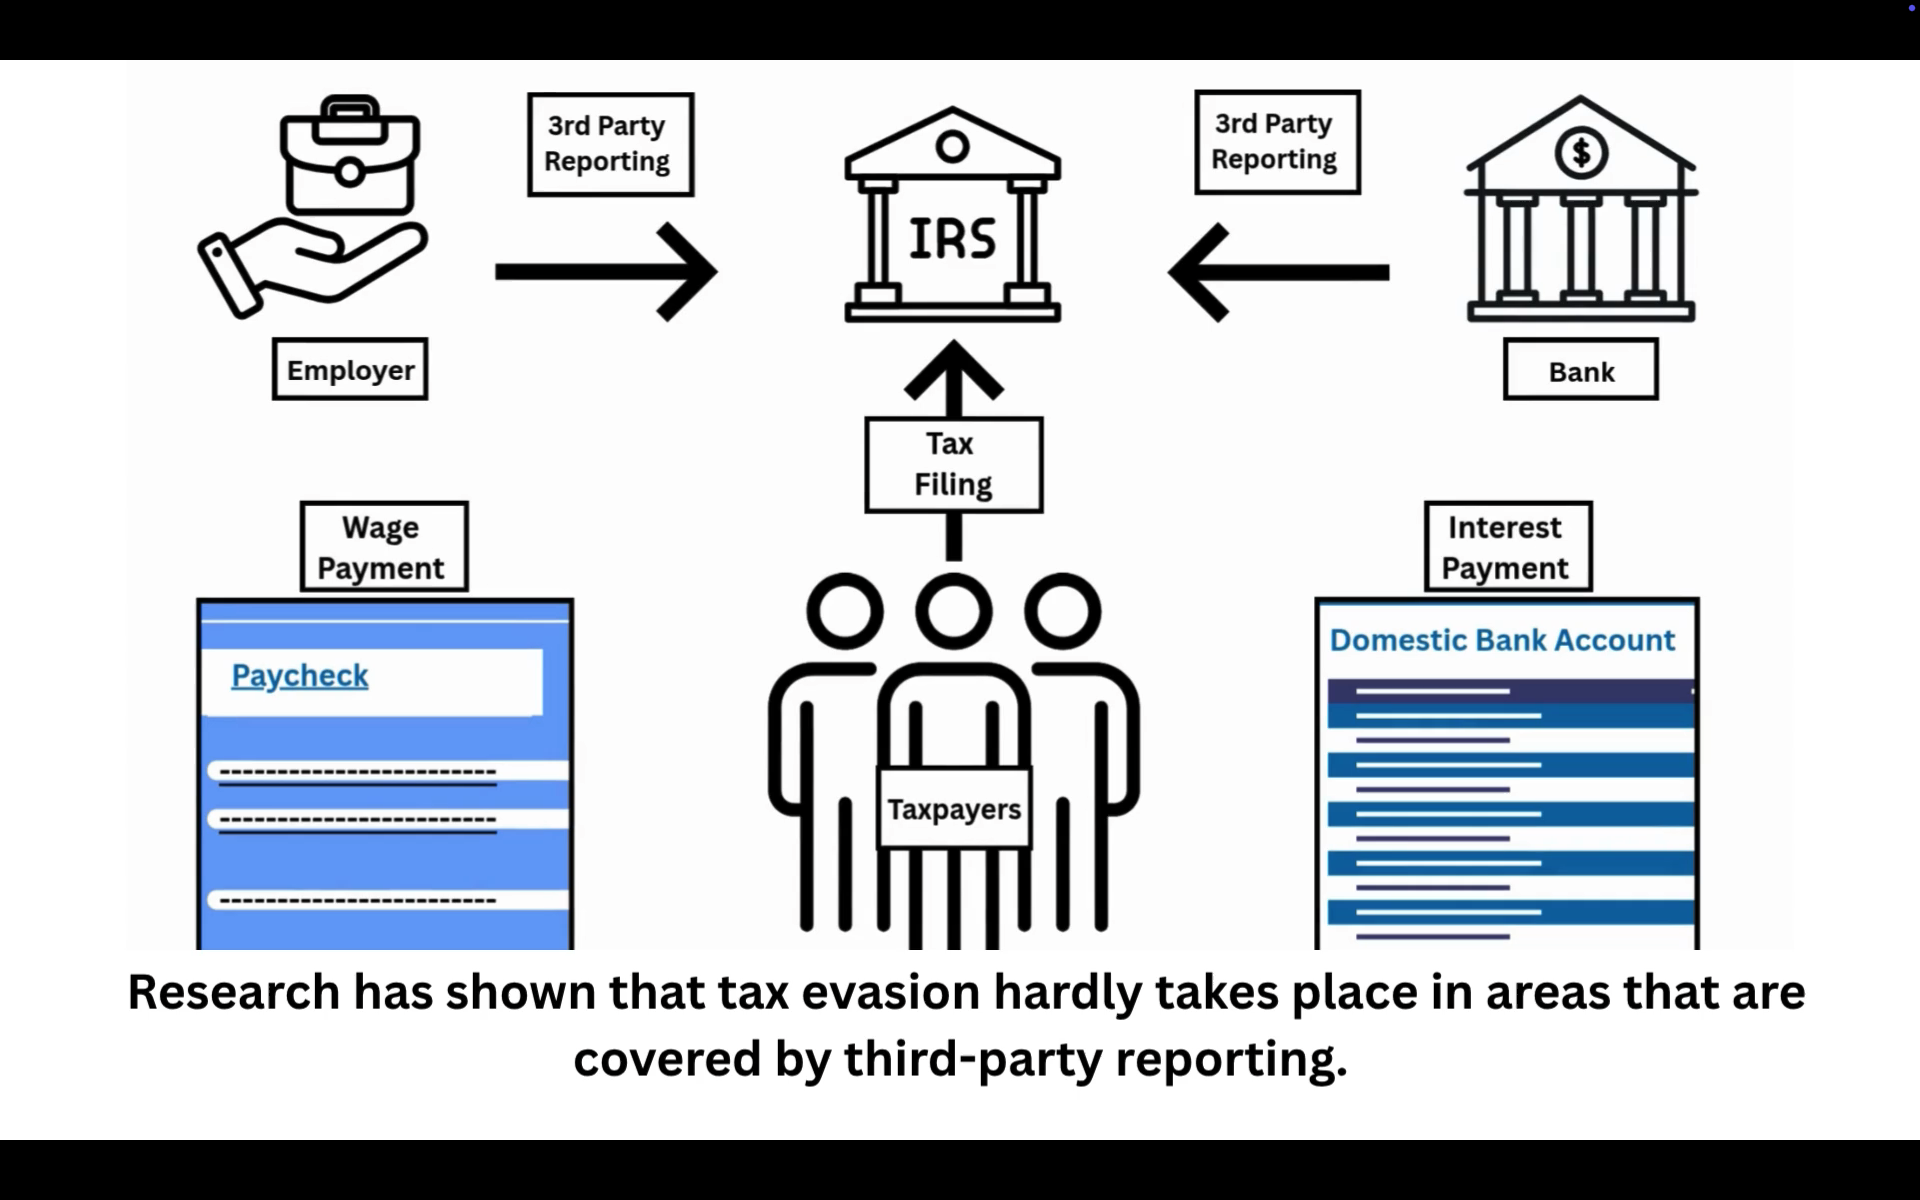
\includegraphics[width=\linewidth, trim={0.5cm 2.5cm 0.5cm 2.5cm}, clip]{Figures_Slides/Revenue_2.png}%
}\\[0.5cm]
\hfill \hyperlink{frame:treatments}{\beamergotobutton{Back}}
  \end{column}
\end{columns}
\end{frame}

\begin{frame}{Filing Costs}
\label{frame:Taxfiling}
\begin{columns}[T] % align columns at the top
  \begin{column}{0.45\textwidth} % left side for text
    \begin{itemize}
    \item Information about economic problem
    \begin{itemize}
        \vspace{0.25em} 
        \item \alert{Tax filing costs}\footnote{\cite{IRS2022}}
    \end{itemize}
    \vspace{2.5em} 
    \item Information about policy
    \begin{itemize}
        \vspace{0.25em} 
        \item Tax software and prepopulated tax returns \alert{reduce tax filing costs}.
        \vspace{0.25em} 
        \item Third-party reporting is \alert{important for prepopulated returns}.\footnote{\cite{goodman2023automated}}
        \vspace{1em}
    \end{itemize}
    \end{itemize}
  \end{column}
  
  \begin{column}{0.45\textwidth} % right side for image
    %\vspace{0.3cm}
    \centering
    \vspace{-0.5em}
    \fbox{%
  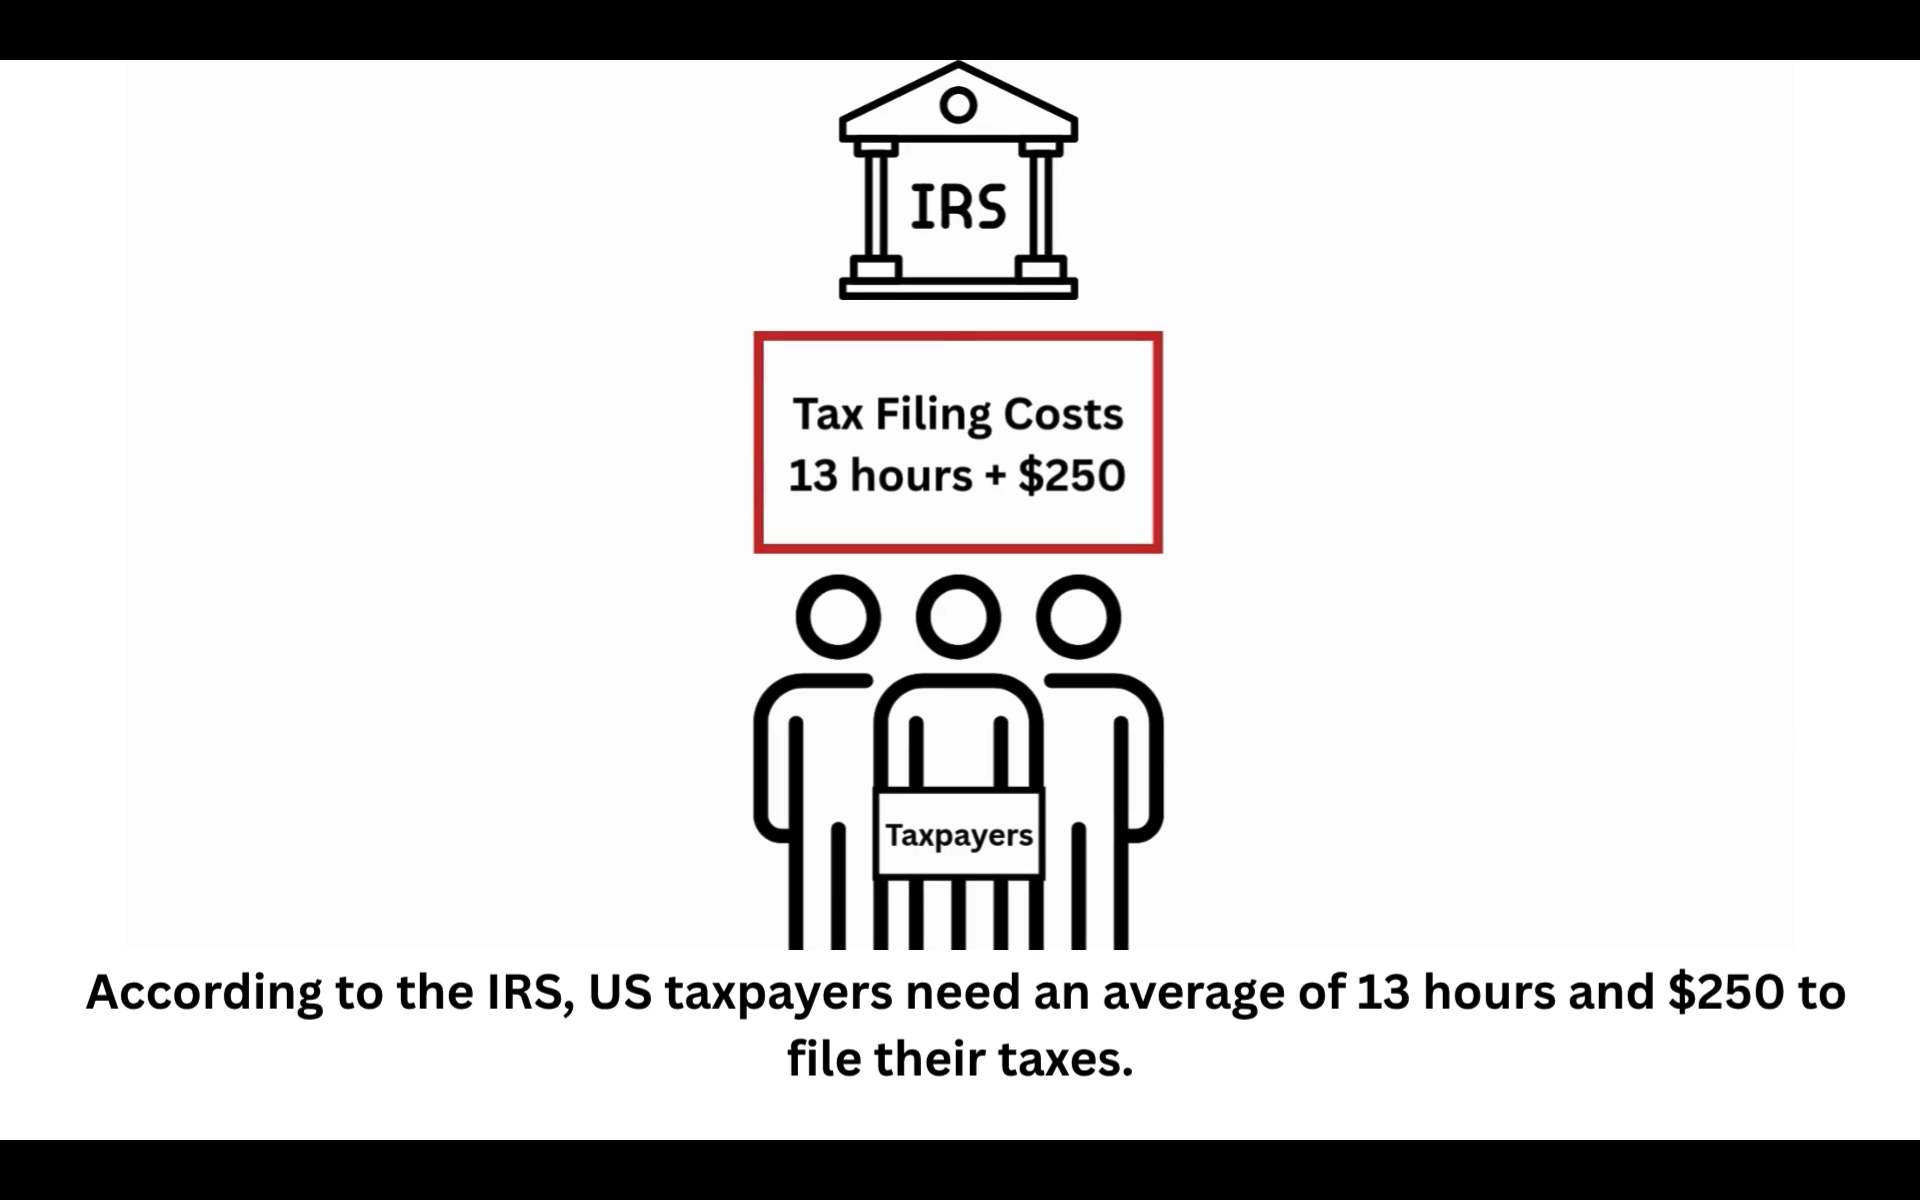
\includegraphics[width=\linewidth, trim={0.5cm 2.5cm 0.5cm 2.5cm}, clip]{Figures_Slides/Filing_3.png}%
}\\[0.5cm]
    %\vspace*{1cm}
\fbox{%
  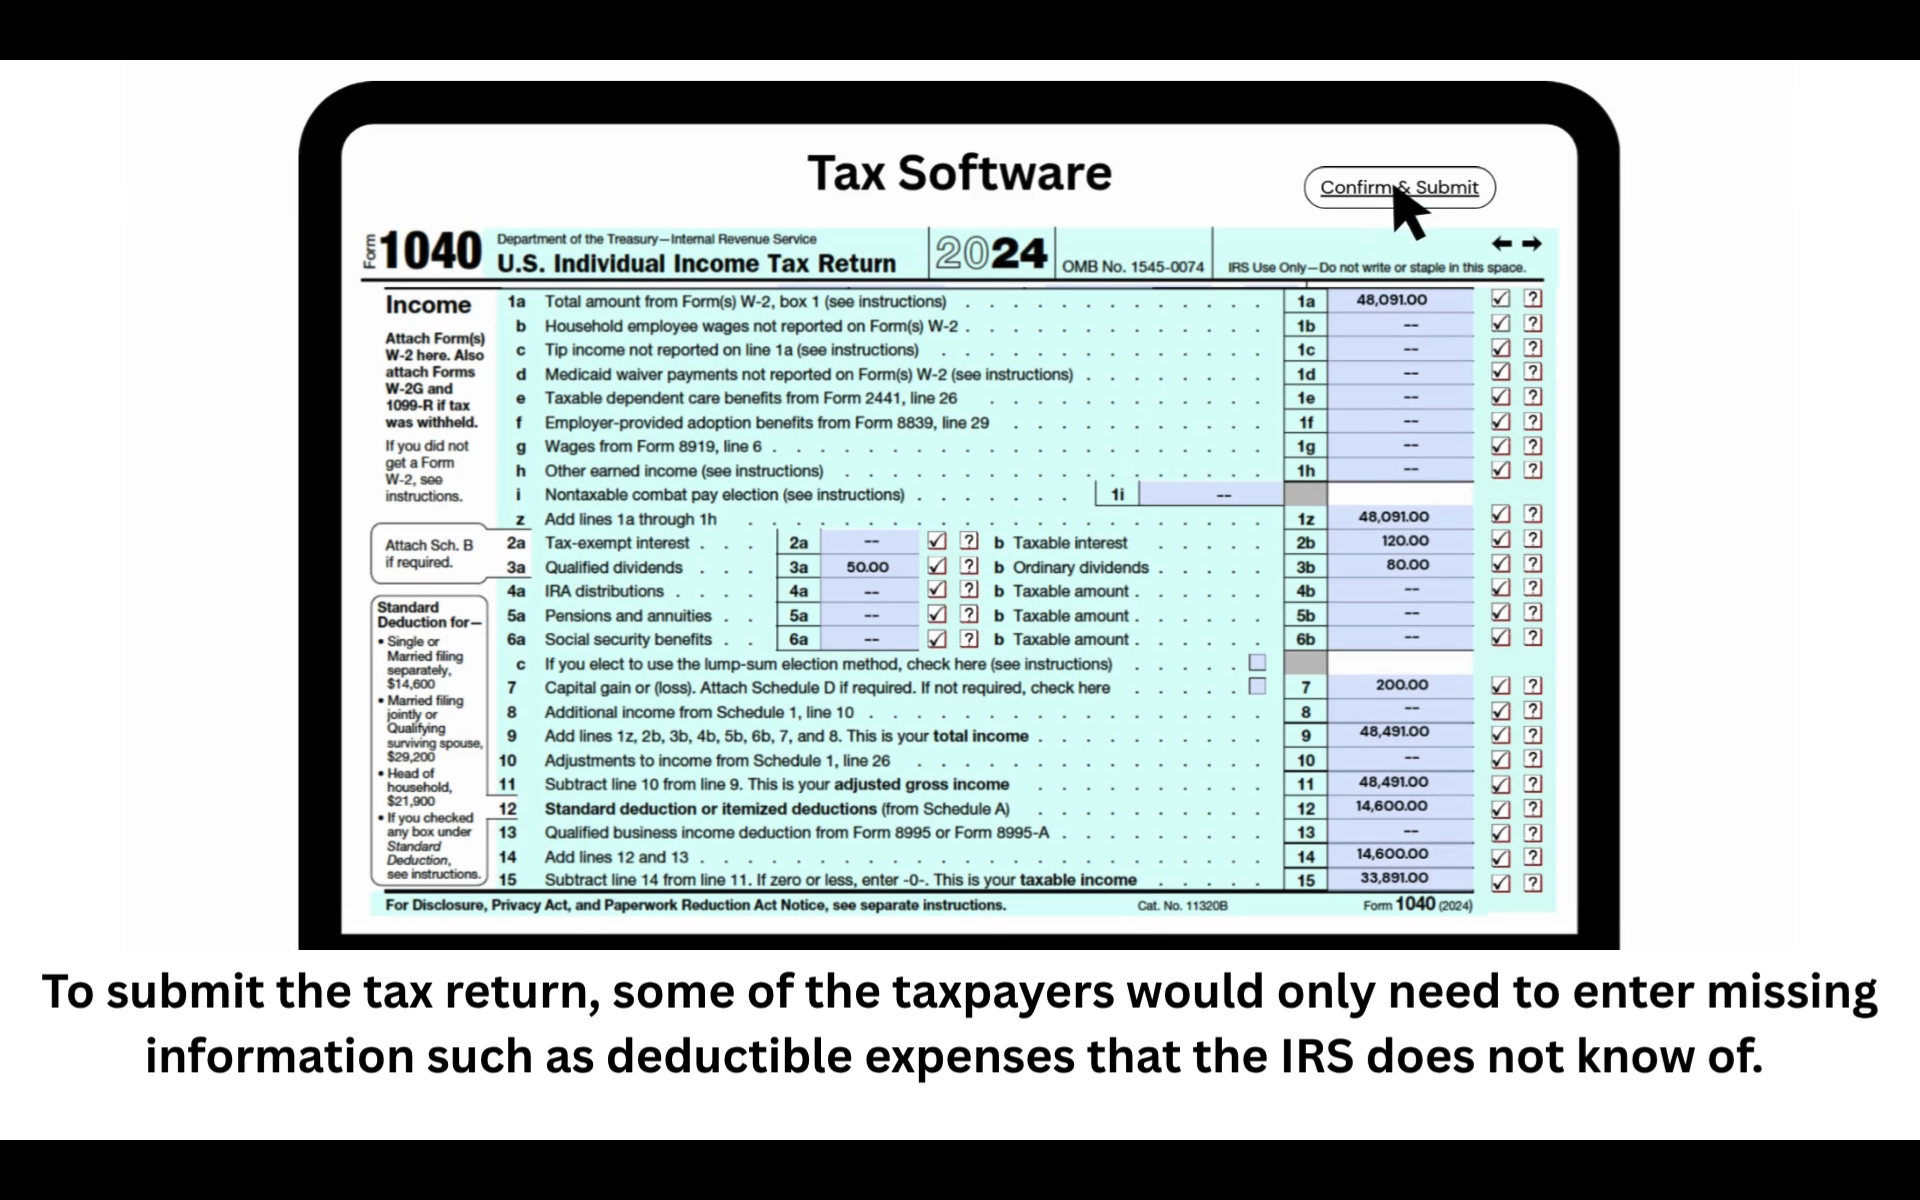
\includegraphics[width=\linewidth, trim={0.5cm 2.5cm 0.5cm 2.5cm}, clip]{Figures_Slides/Filing_1.png}%
}\\[0.5cm]
\hfill \hyperlink{frame:treatments}{\beamergotobutton{Back}}
  \end{column}
\end{columns}
\end{frame}

\begin{frame}{Full Info}
\label{frame:Fullinfo}
\begin{columns}[T] % align columns at the top
  \begin{column}{0.35\textwidth} % right side for image
    %\vspace{0.3cm}
    \centering
    Filing Treatment
    \vspace{-0.5em}
    \fbox{%
  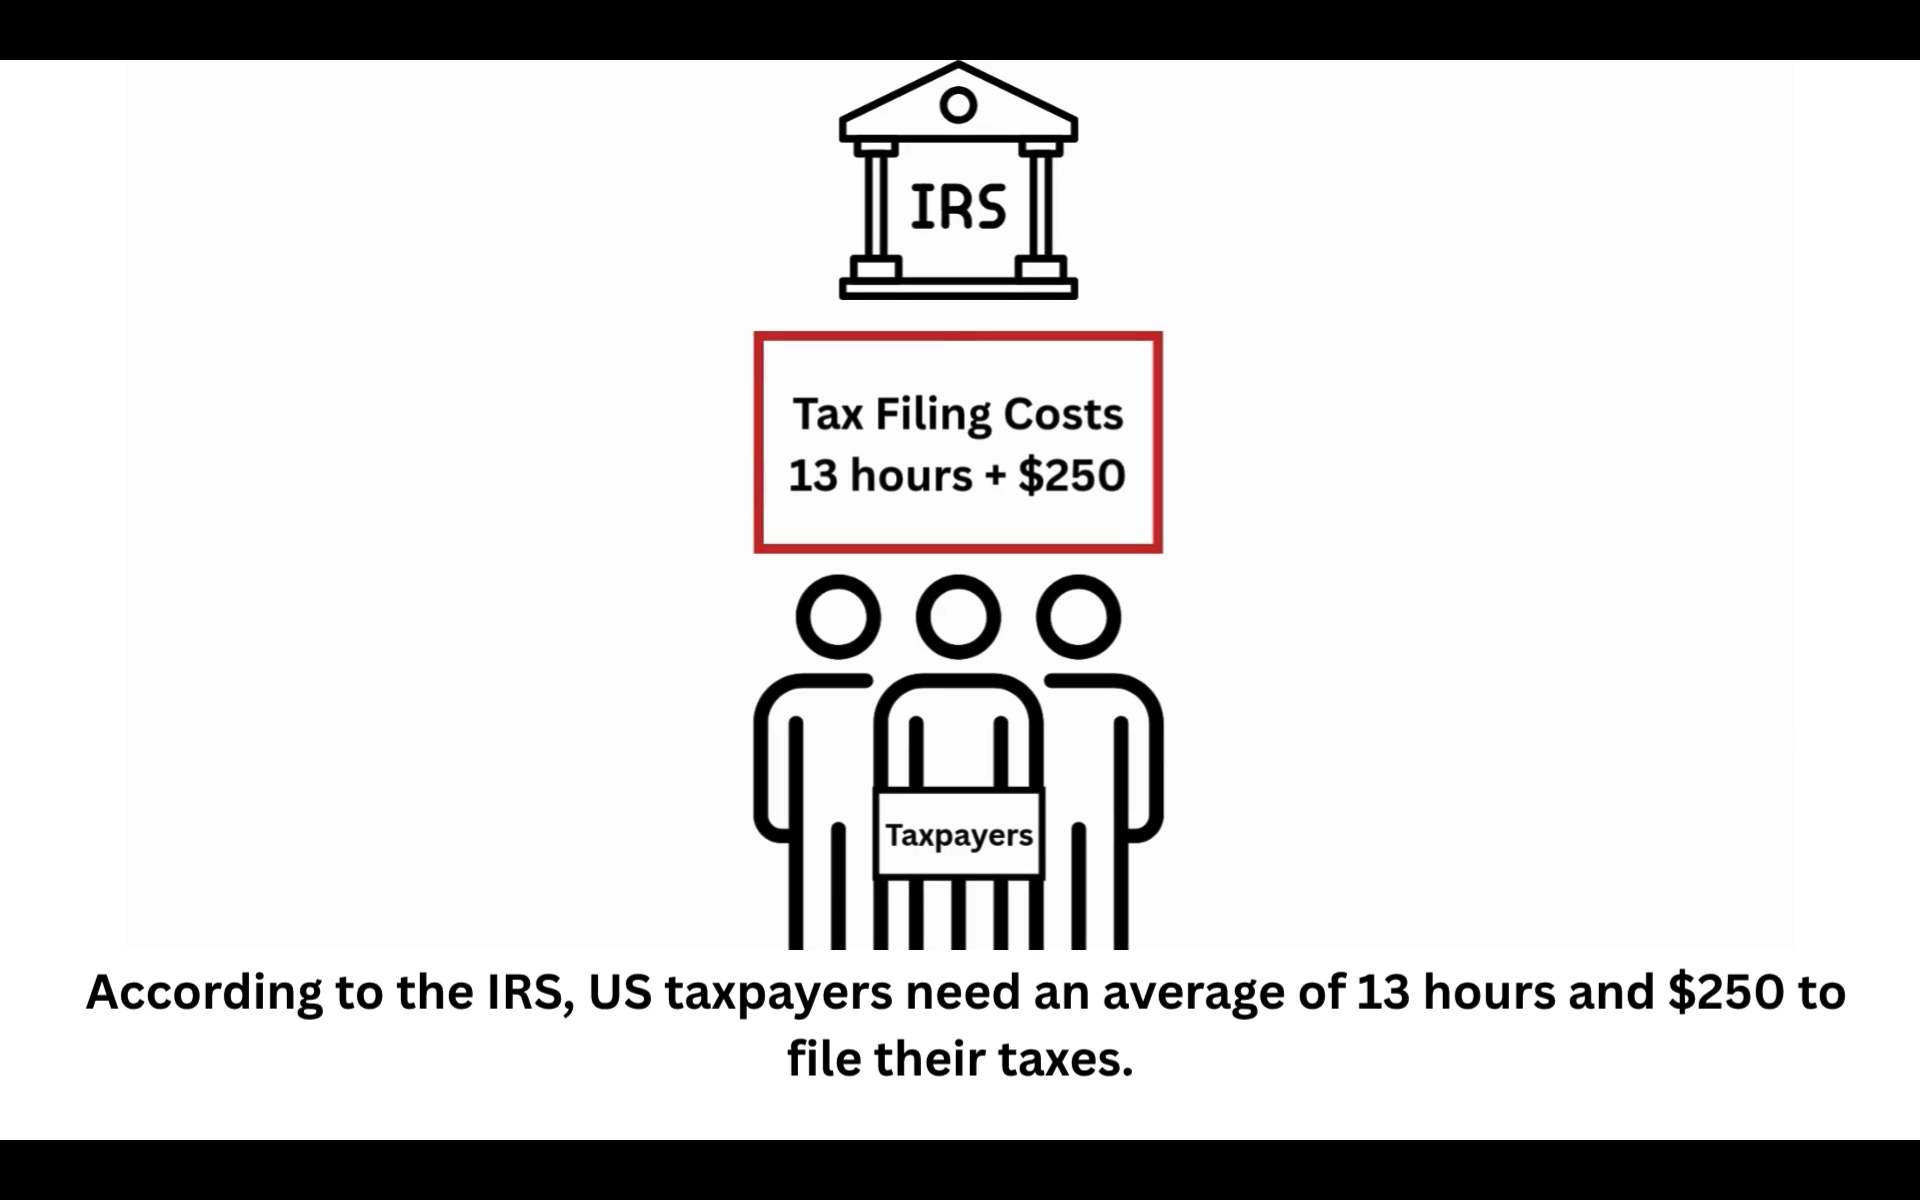
\includegraphics[width=\linewidth, trim={0.5cm 2.5cm 0.5cm 2.5cm}, clip]{Figures_Slides/Filing_3.png}%
}\\[0.5cm]
    %\vspace*{1cm}
\fbox{%
  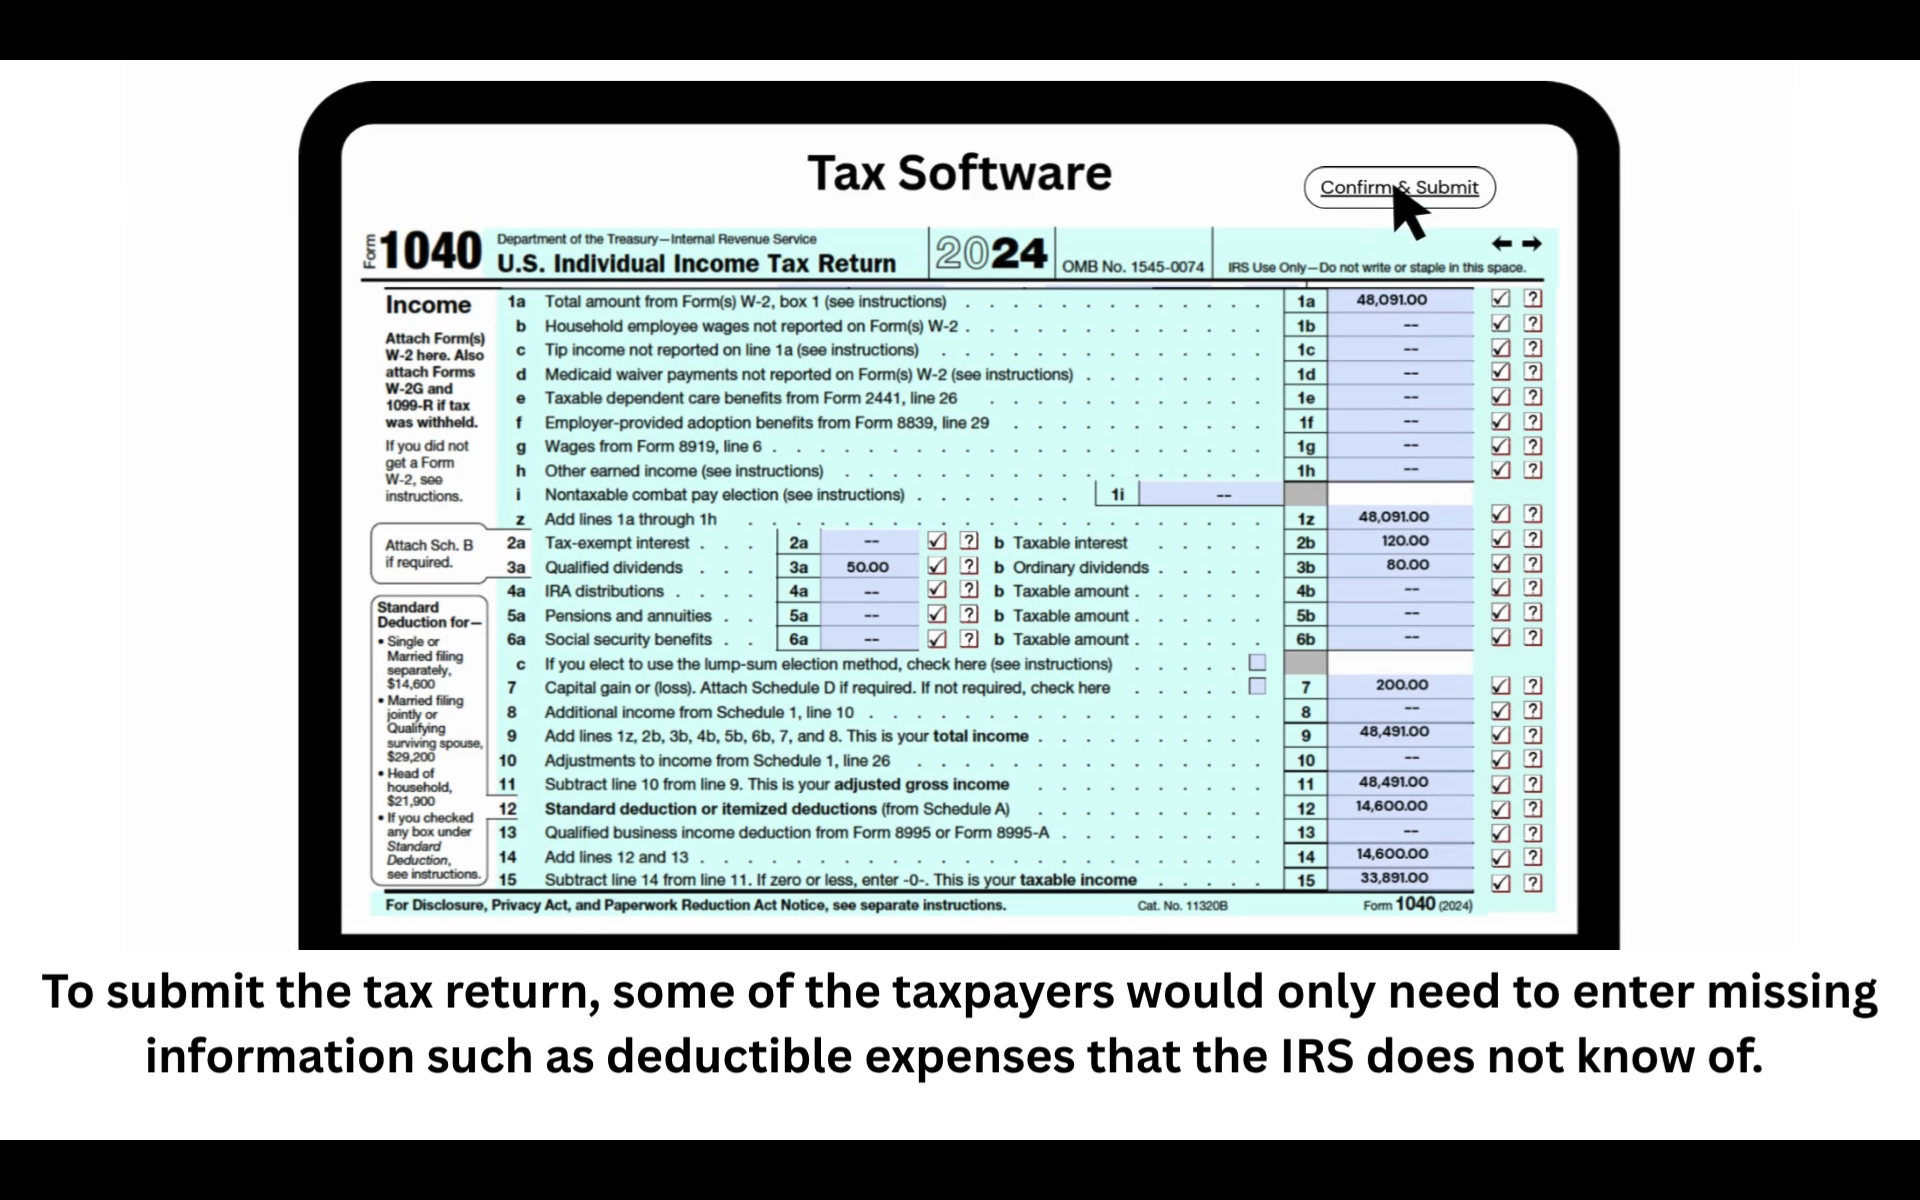
\includegraphics[width=\linewidth, trim={0.5cm 2.5cm 0.5cm 2.5cm}, clip]{Figures_Slides/Filing_1.png}%
}
  \end{column}
  \begin{column}{0.05\textwidth}
  \centering
  \vspace{2cm}
  \Large $\longrightarrow$
\\[0.5cm]
\Large $\longrightarrow$
\\[0.5cm]
\Large $\longrightarrow$
  \end{column}
  \begin{column}{0.35\textwidth} % left side for text
    %\vspace{0.3cm}
    \centering
      Inequality Treatment
    \vspace{-0.5em}
    \fbox{%
  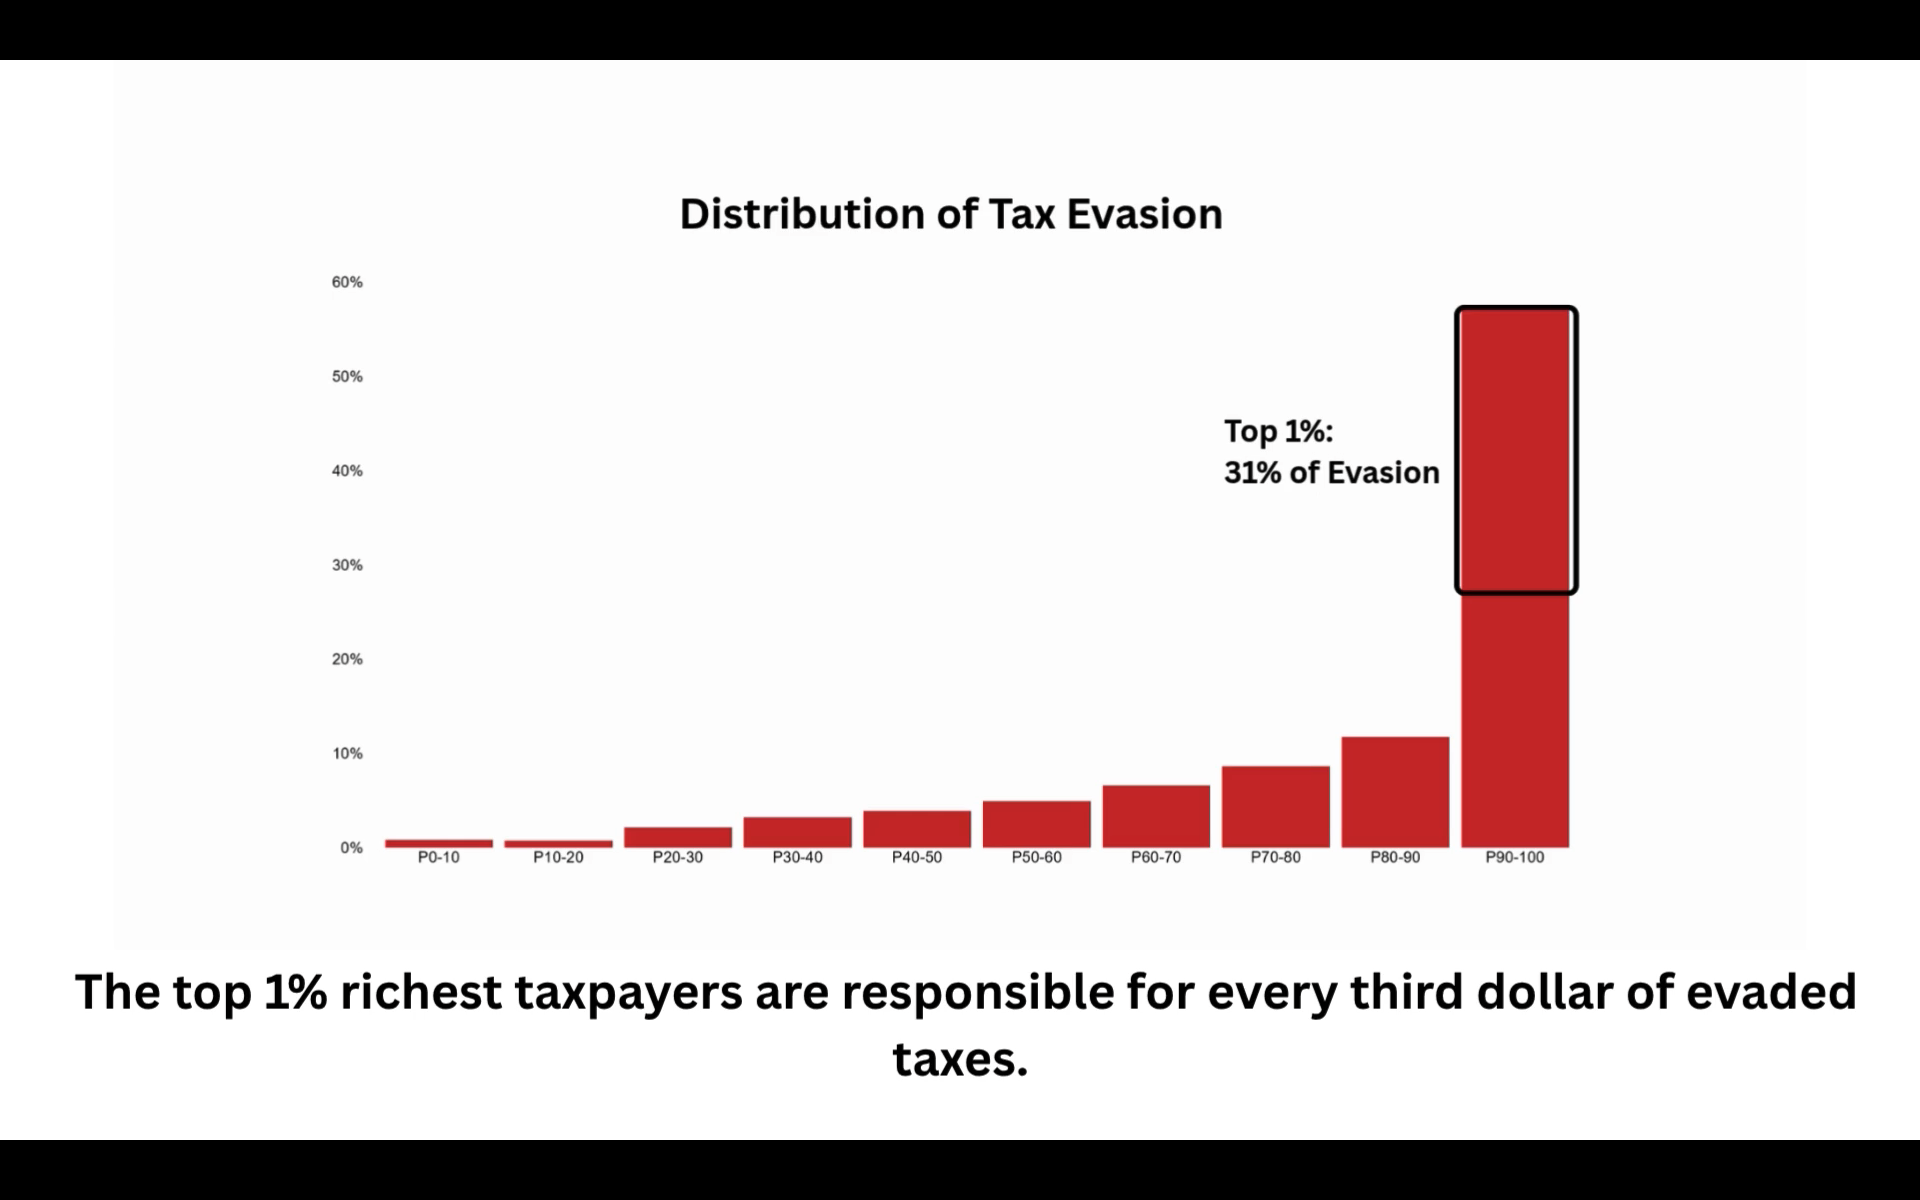
\includegraphics[width=\linewidth, trim={0.5cm 2.5cm 0.5cm 2.5cm}, clip]{Figures_Slides/Inequality_1.png}%
}\\[0.5cm]
    %\vspace*{1cm}
\fbox{%
  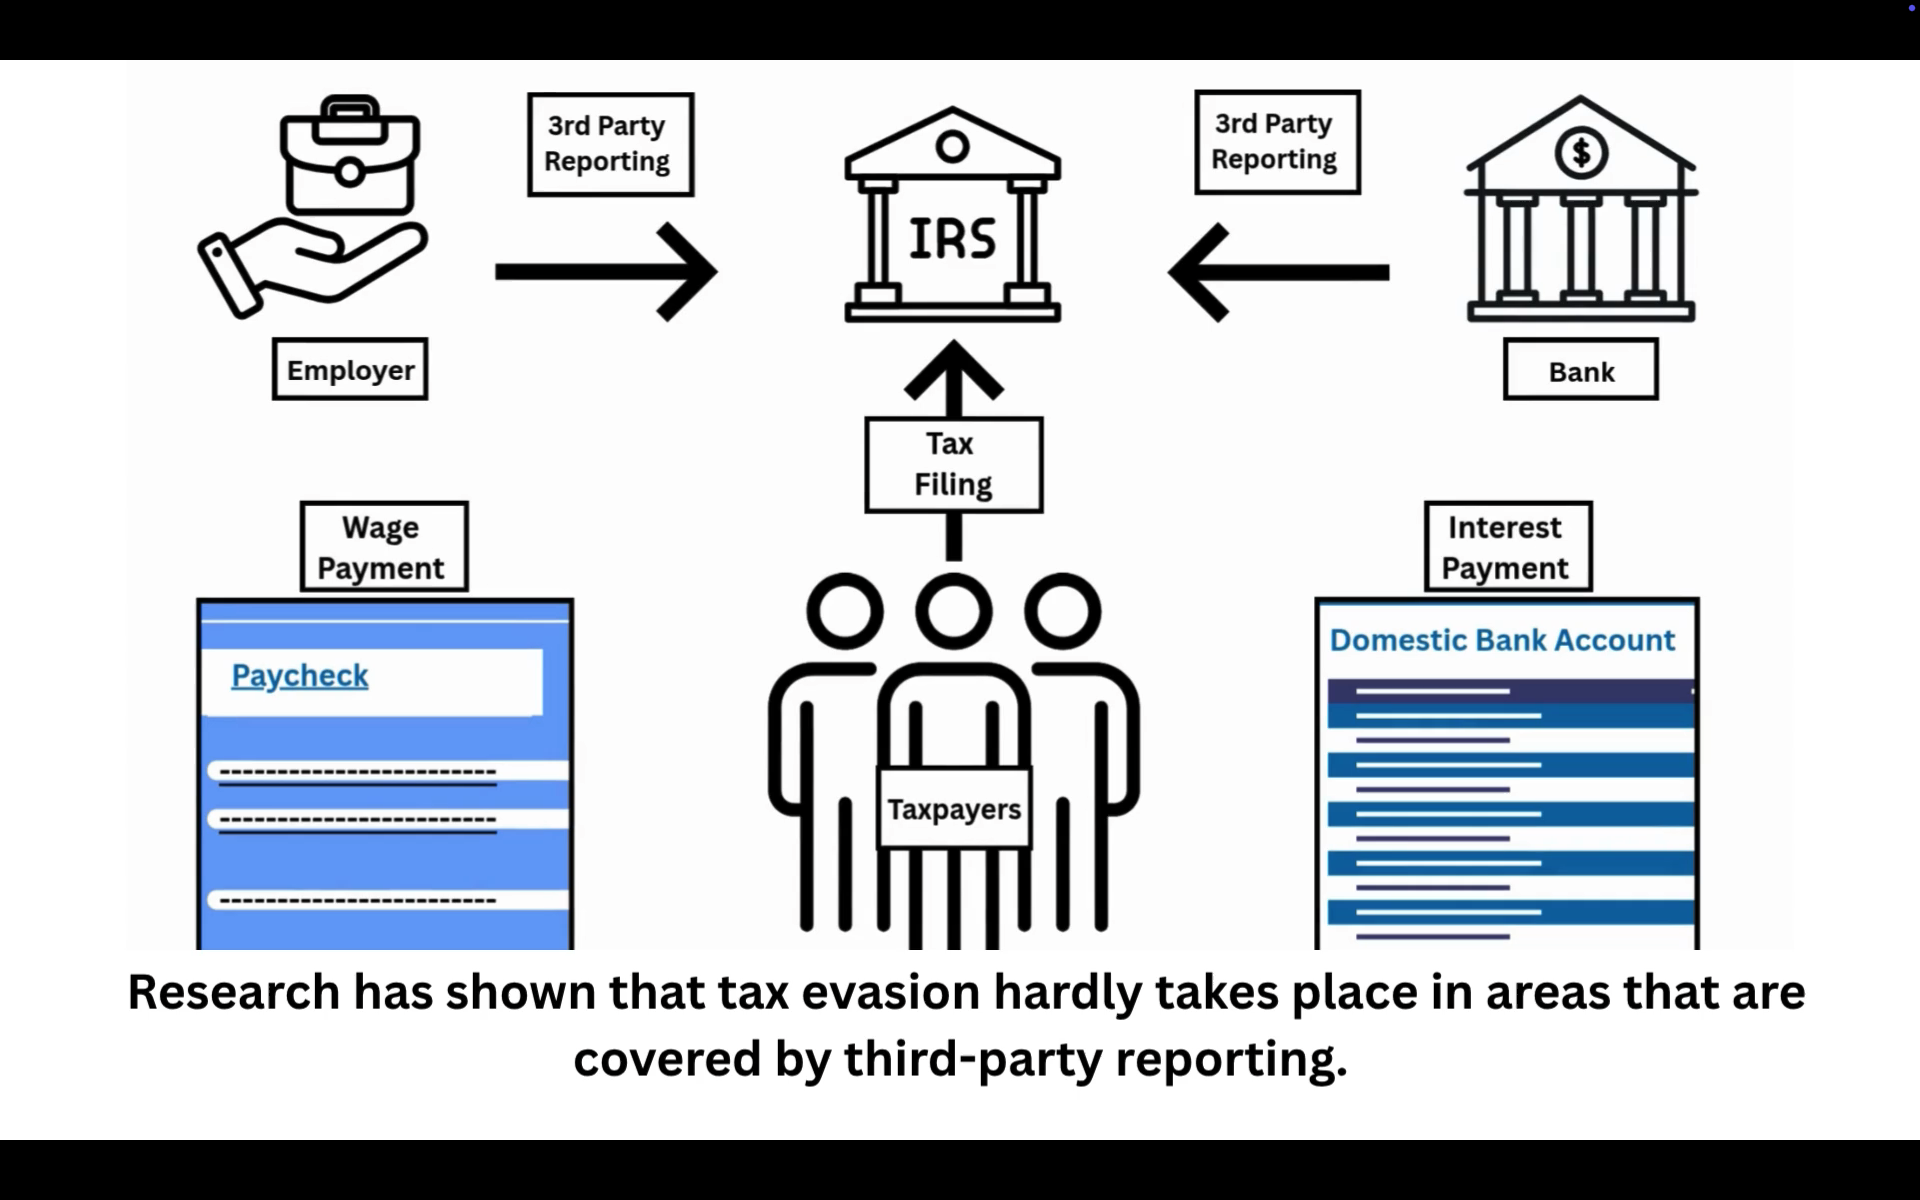
\includegraphics[width=\linewidth, trim={0.5cm 2.5cm 0.5cm 2.5cm}, clip]{Figures_Slides/Revenue_2.png}%
}
  \end{column}

\end{columns}
\vspace{0.3cm}
\centering

\hfill \hyperlink{frame:treatments}{\beamergotobutton{Back}}
\end{frame}


%\begin{frame}[label=Prior_Perceptions]{Perceptions about Underlying \\ Factors}
%\begin{columns}[T] % align columns at the top
%  \begin{column}{0.45\textwidth} % left side for text
%    \begin{itemize}
%    \item Perception about the tax gap
%    \vspace{0.5em} 
%    \item Perception about tax filing cost
%    \begin{itemize}
%        \item time
%        \item monetary cost
%    \end{itemize}
%    \vspace{2em} 
%    \item[$\Rightarrow$] Understand whether respondents update perceptions. 
%    \end{itemize}
%  \end{column}
%  
%  \begin{column}{0.45\textwidth} % right side for image
%    \centering
%     \vspace{-4em}
%    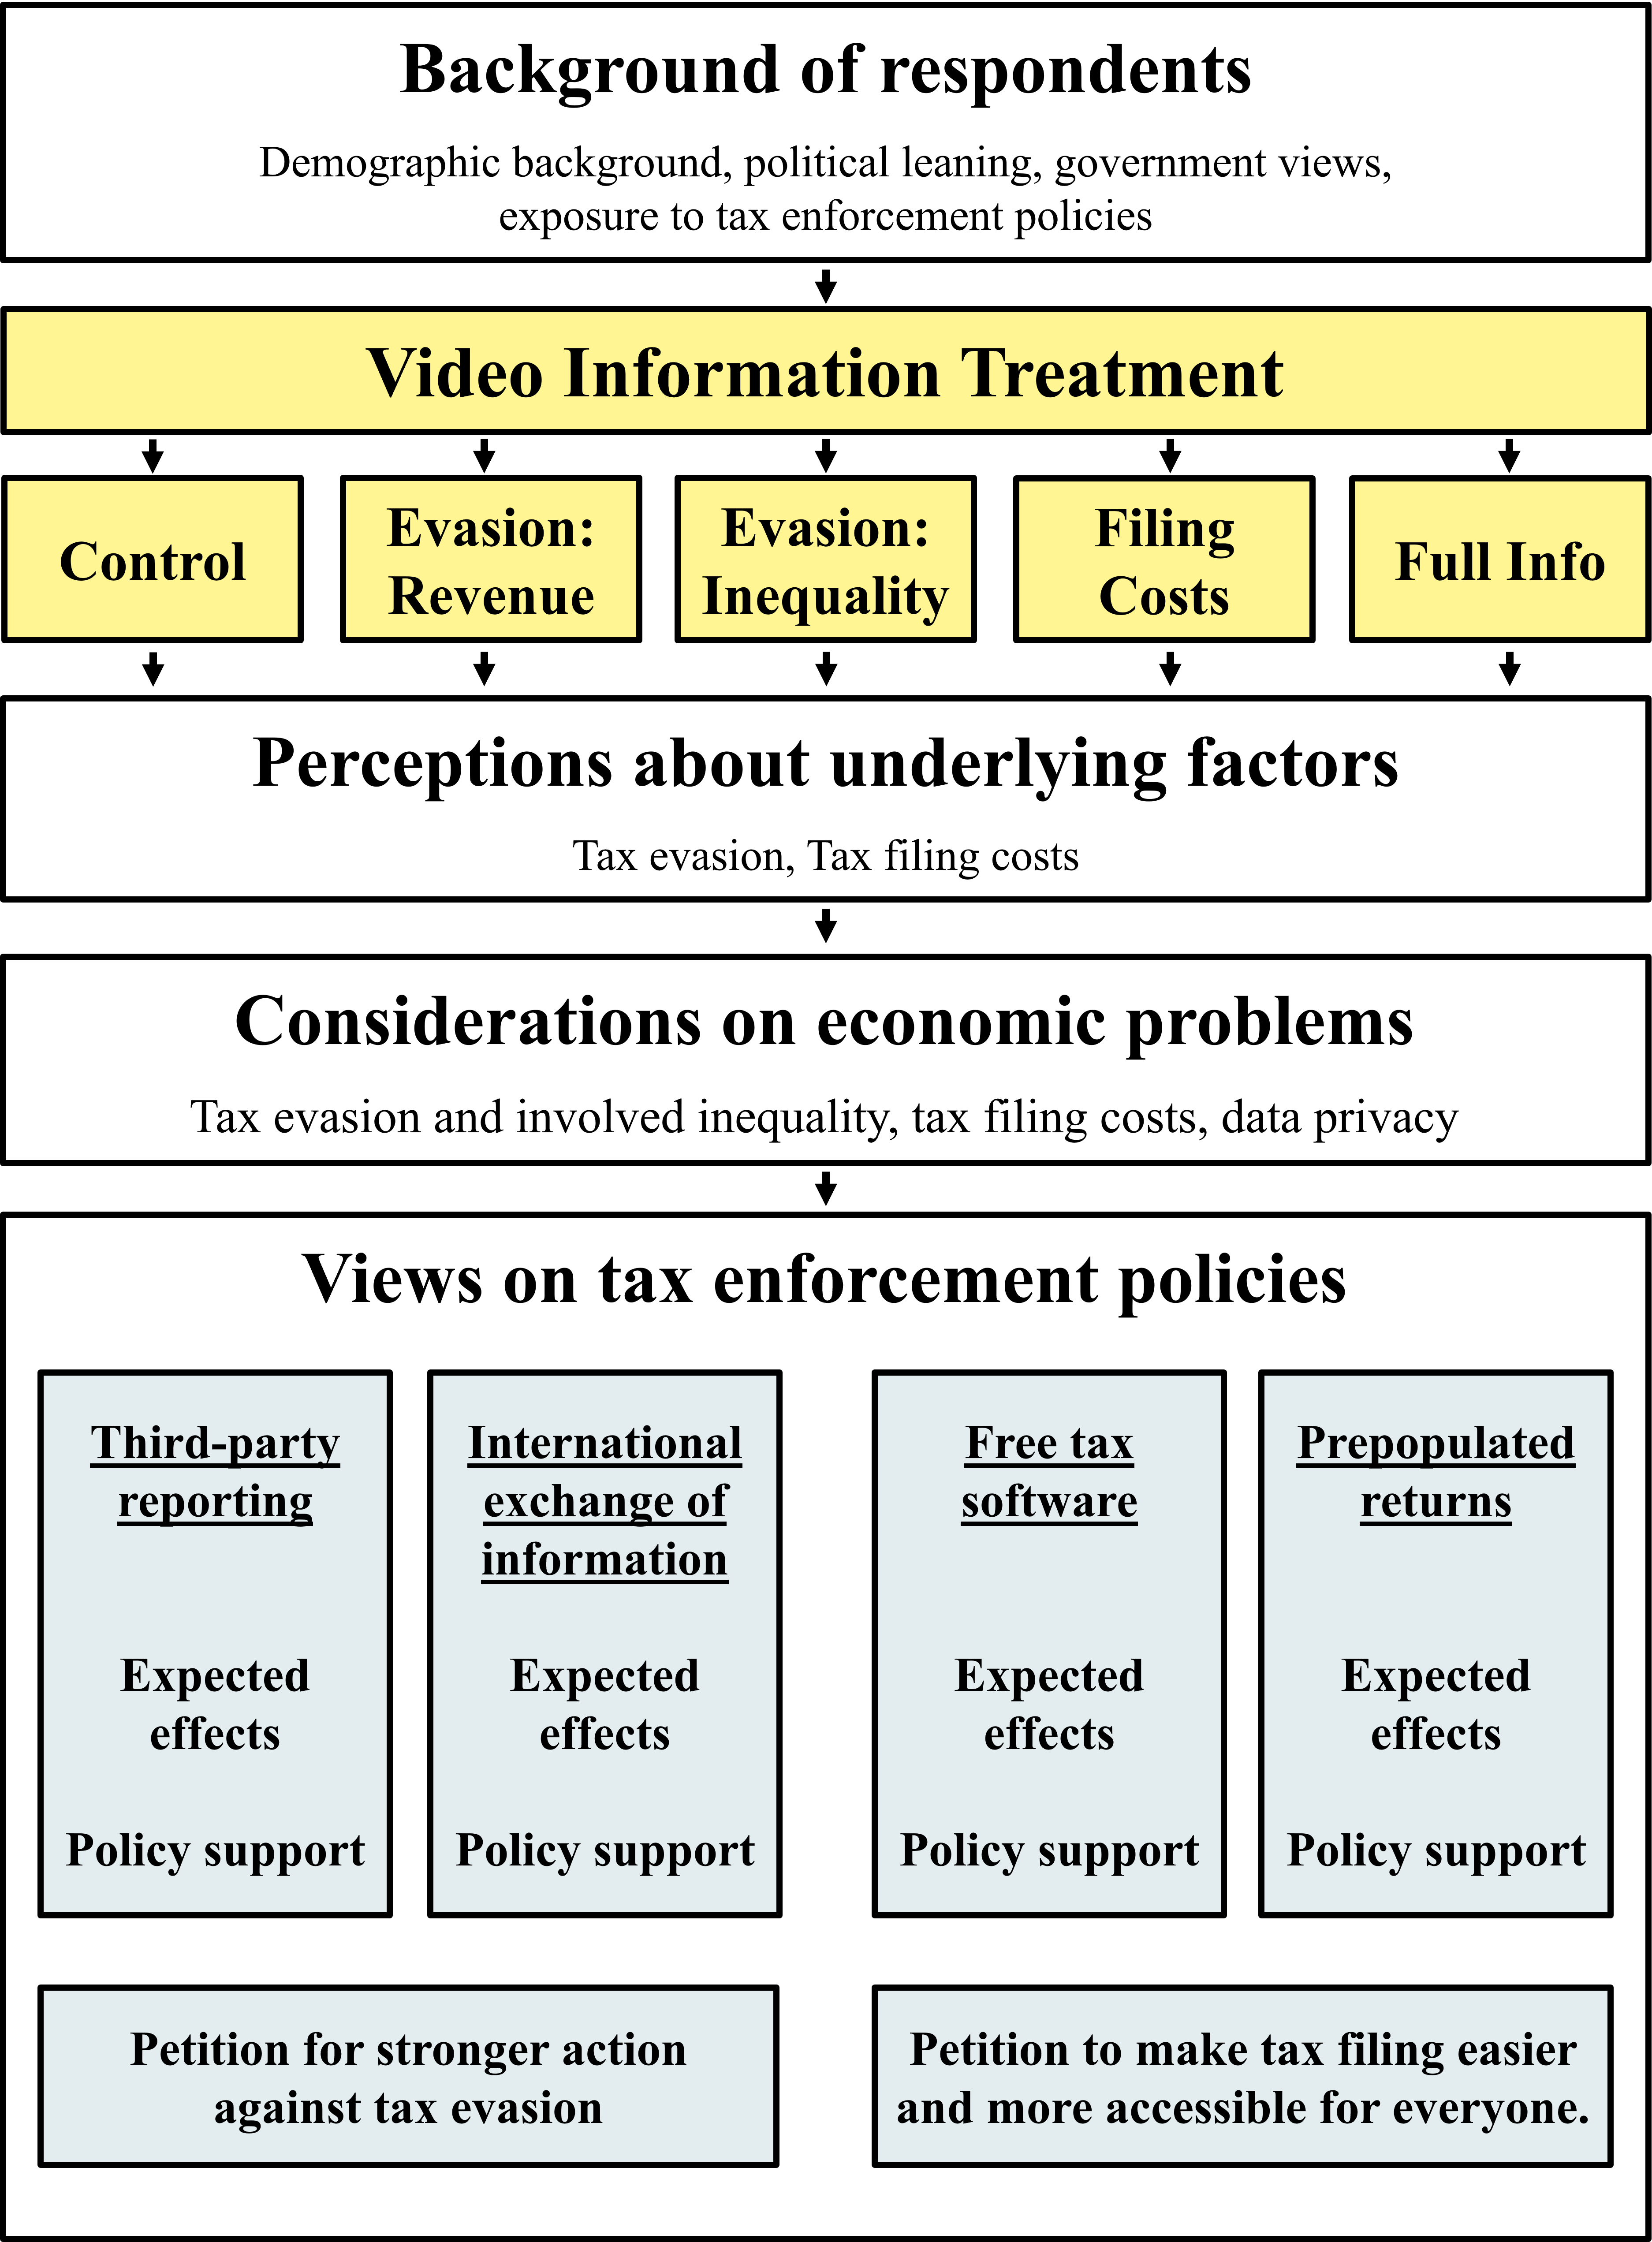
\includegraphics[width=1.05\linewidth]{Figures_Slides/Survey_Overview_Treatments.png}
%  \end{column}
%\end{columns}
%\end{frame}

%\begin{frame}[label=General_Considerations]{General Considerations \hyperlink{General_Considerations_Appendix}{\beamergotobutton{A: GC}}}
%\begin{columns}[T] % align columns at the top
%  \begin{column}{0.45\textwidth} % left side for text
%    \begin{itemize}
%    \item Tax system 
%    \begin{itemize}
%        \item Is it fair? 
%    \end{itemize}
%    \vspace{0.2em} 
%    \item Tax evasion
%    \begin{itemize}
%        \item Is it concerning? 
%        \item Is it important for the government to reduce it?
%    \end{itemize}
%    \vspace{0.2em} 
%    \item Tax filing costs
%    \begin{itemize}
%        \item Are they concerning? 
%        \item Is it important for the government to reduce them?
%    \end{itemize}
%    \vspace{0.2em} 
%    \item Data privacy
%    \begin{itemize}
%        \item Is it a problem if the government collects data on citizens?
%    \end{itemize}
%    \end{itemize}
%  \end{column}
%  
%  \begin{column}{0.45\textwidth} % right side for image
%    \centering
%     \vspace{-2em}     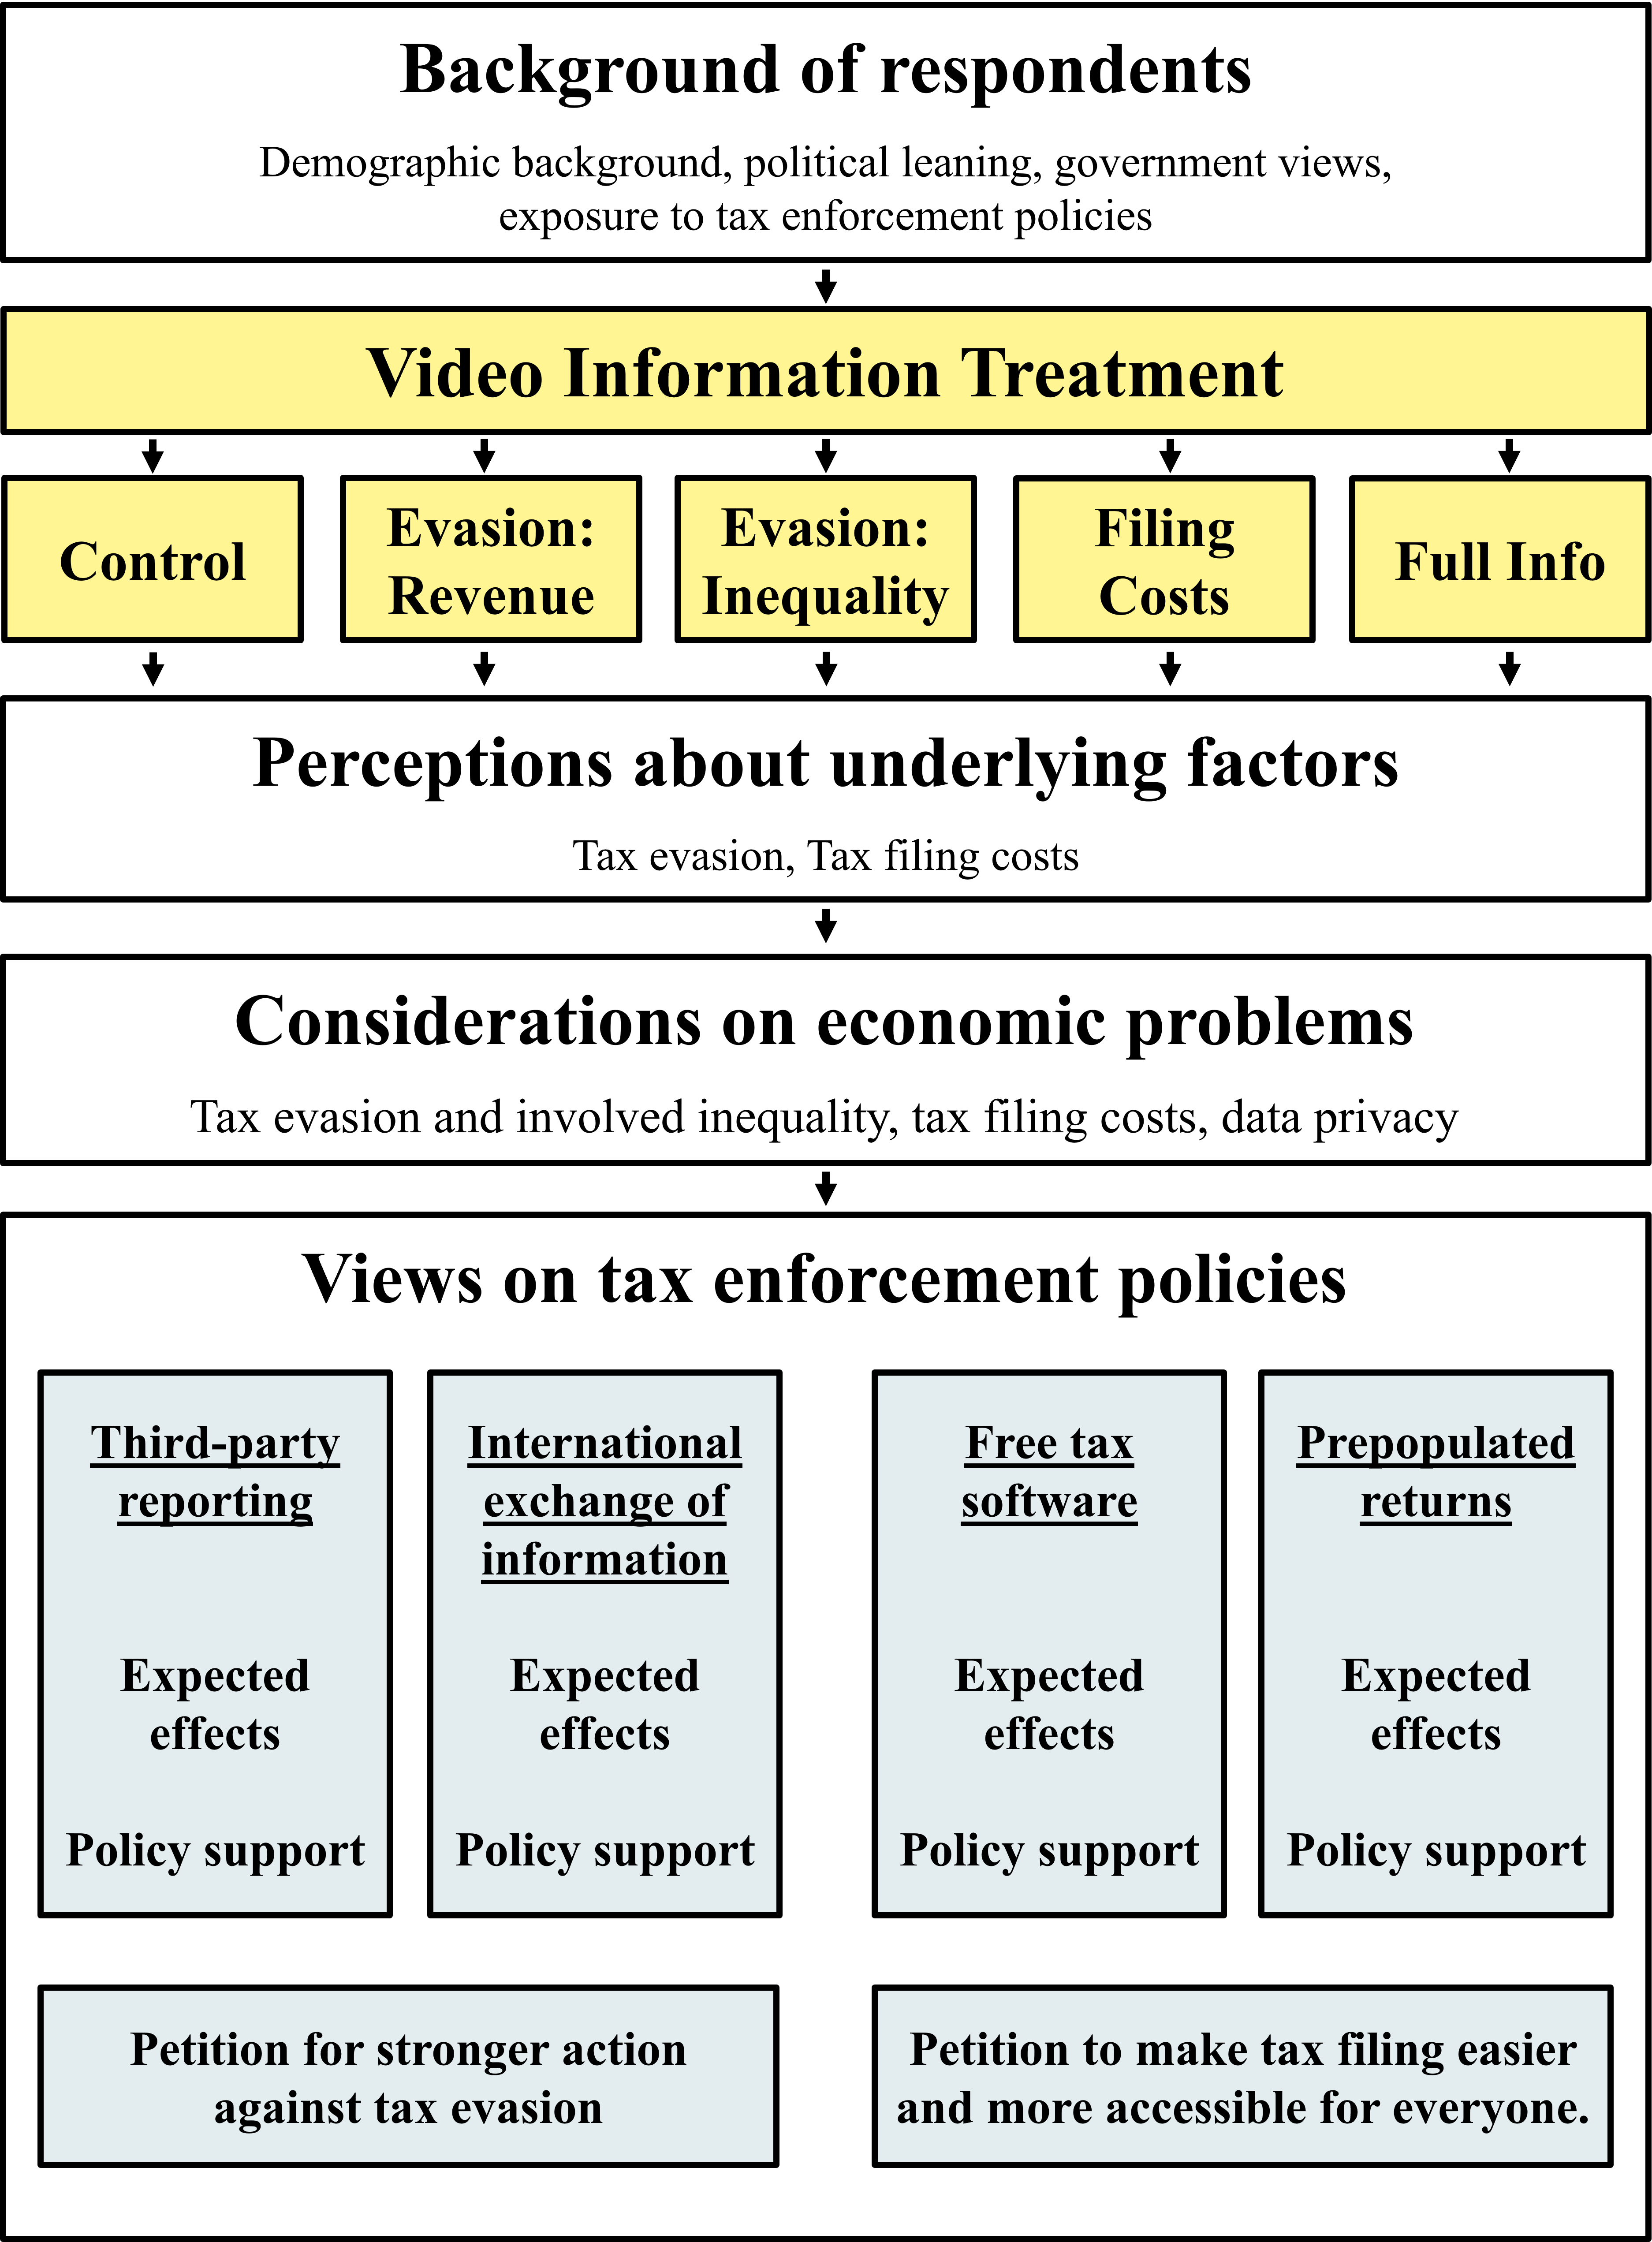
\includegraphics[width=1.05\linewidth]{Figures_Slides/Survey_Overview_Treatments.png}
%  \end{column}
%\end{columns}
%\hfill
%\vfill
%\end{frame}

\begin{frame}[label=Third_Party_Reporting]
  \begin{center}
 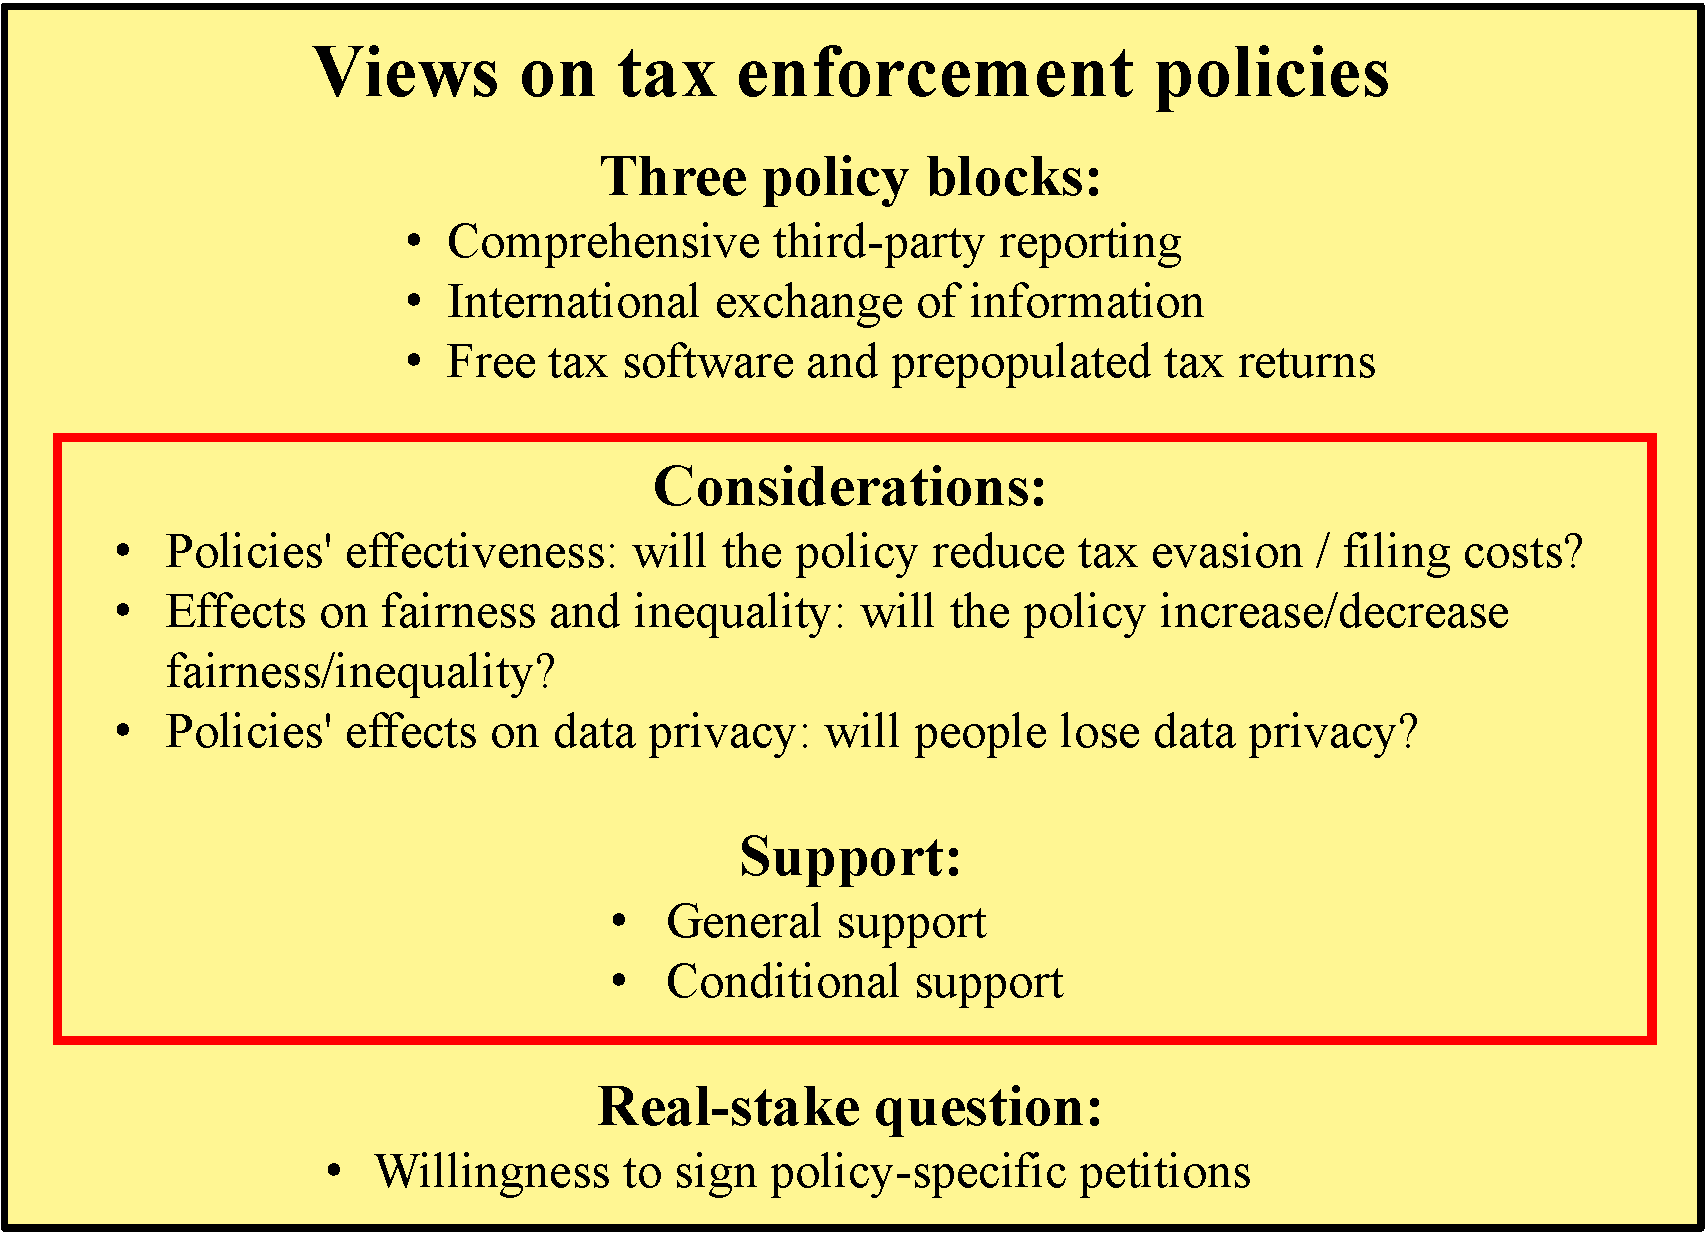
\includegraphics[width=0.65\textwidth]{Figures_Slides/Survey_Overview_Policy_Views_1.pdf} \\
  \end{center}
  %\vspace{0.1cm}
  \begin{center}
 % <-- Breite nach Wunsch anpassen
    The structure of the questionnaire is the same for each policy. \hyperlink{Third_Party_Reporting_Appendix}{\beamergotobutton{A: TPR}}
    \end{center}
    \begin{center}
\begin{minipage}{0.65\textwidth}

    \begin{enumerate}
        \item Short introduction to the policy.
        \item Policy-related considerations/expectations.
        \item Policy support. (general \& conditional)
    \end{enumerate}
  \end{minipage}
  \end{center}
\end{frame}

\begin{frame}[label=Petitions]
  \begin{center}
    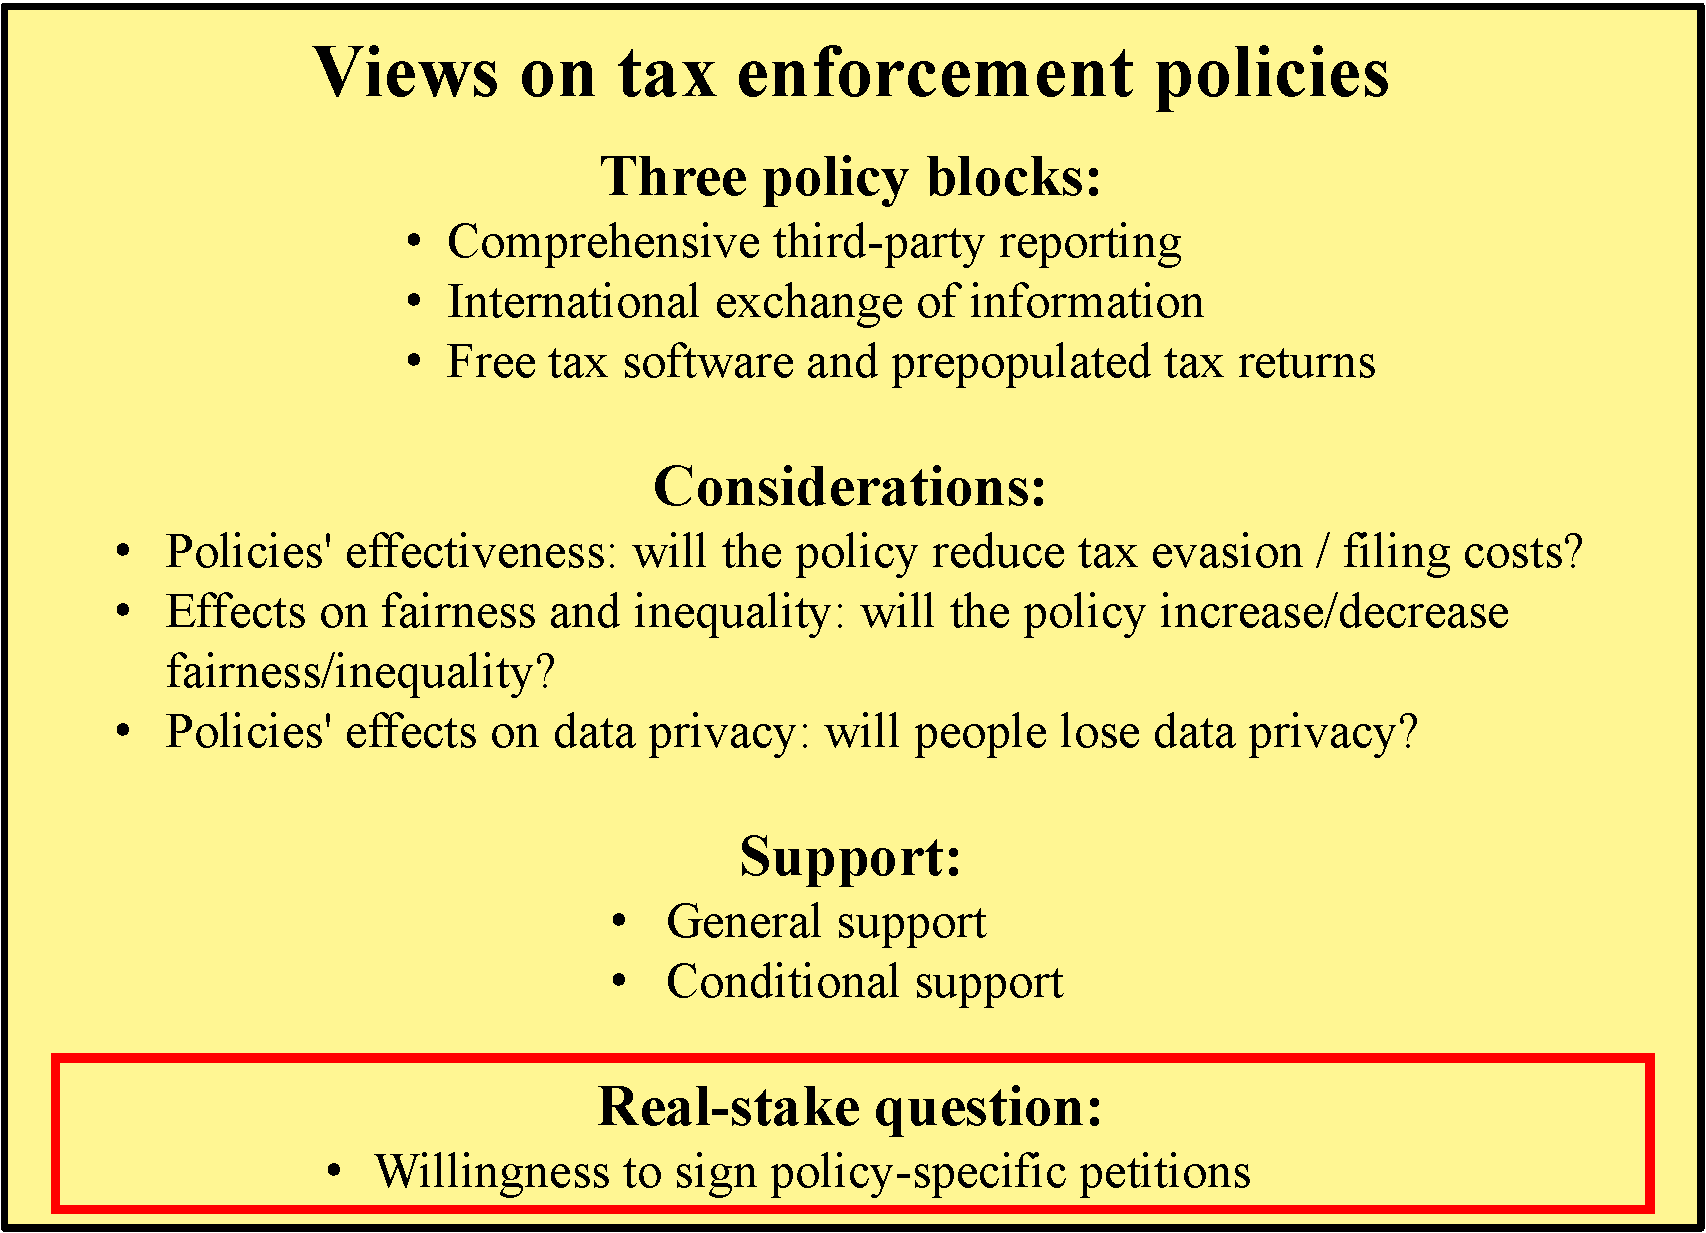
\includegraphics[width=0.65\textwidth]{Figures_Slides/Survey_Overview_Policy_Views_2.pdf} \\
  \end{center}

  

We ask respondents if they want to support \alert{petitions} that aim at policies very similar to our policies from the survey.  \hyperlink{Petitions_Appendix}{\beamergotobutton{A: Petitions}}

  \footnotesize % make the font smaller only for the table
  \begin{tabularx}{\textwidth}{*{2}{>{\centering\arraybackslash}X}}
    \begin{enumerate}
      %\item TPR$^{+}$ $\times$ \\Tax evasion$^{-}$
      \item \alert{in favor} of comprehensive \alert{third- party reporting} to act against tax evasion.
    \end{enumerate} &
    %\begin{enumerate}
    %\setcounter{enumi}{1} % start at 2
    %  %\item TPR$^{-}$ $\times$ \\Data privacy$^{+}$
    %  \item \alert{against} comprehen- sive \alert{third-party reporting} in order to protect privacy.
    %\end{enumerate} &
    \begin{enumerate}
    \setcounter{enumi}{1} % start at 2
      %\item Filing services$^{+}$ $\times$ \\Filing costs$^{-}$
      \item \alert{in favor of making tax filing easier} and more accessible for everyone.
    \end{enumerate} \\
  \end{tabularx}
  \normalsize % reset font size after the table
\end{frame}

\begin{frame}{What are Peoples' Considerations on Economic Problems?}
\label{Example:ConsiderationsEconomicProblems}
\begin{table}[!htbp]\centering
\tiny
\caption{Considerations on economic problems}
\begin{threeparttable}
\begin{tabular}{l|ccc|cc|c}
\toprule
 & \multicolumn{3}{c}{Tax evasion} & \multicolumn{2}{c}{Filing costs} & Data privacy\\
 & is a serious &is unequally & is important & are & are important  & is important  \\
  &  problem & distributed & to reduce & high& to reduce & to protect  \\
\midrule
Female                     &-& - & - &-& - & -  \\
Age                        &-& - & - &-& - & -  \\
College degree             &-& - & - &-& - & -  \\
Middle income              &-& - & - &-& - & -  \\
High income                &-& - & - &-& - & -  \\
Middle wealth              &-& - & - &-& - & -  \\
High wealth                &-& - & - &-& - & -  \\
Self-employed              &-& - & - &-& - & -  \\
Republican                 &-& - & - &-& - & -  \\[1em]
Evasion: Revenue        & - & - & - & - & - & - \\
Evasion: Inequality     & - & - & - & - & - & - \\
Filing costs            & - & - & - & - & - & - \\
Full info               & - & - & - & - & - & - \\[0.5em]
\midrule
Intercept &- &- &- &- &- &-   \\
Observations                        &-    &-    &-    &-    &-    &-         \\
$R^2$                               &-    &-    &-    &-    &-    &-         \\
Controls                 & Yes     & Yes    & Yes    & Yes     & Yes    & Yes      \\
\bottomrule
\end{tabular}
\begin{tablenotes}[flushleft]
%\footnotesize
\item \textit{Notes}: The dependent variable in the first column is the response to the question of whether tax evasion is a serious problem. 
\end{tablenotes}
\end{threeparttable}
\end{table}
\hfill \hyperlink{posttreatment}{\beamergotobutton{Back}}
\end{frame}

\begin{frame}{Example: How Do Beliefs Differ among Respondents?}
\label{Example:ExpectedEffects}
\begin{table}[!htbp]\centering
\tiny
\caption{Expected effects of tax enforcement policy}
\begin{threeparttable}
\begin{tabular}{l|cc|cc|cc|cc|cc|cc}
\toprule
 & \multicolumn{4}{c|}{Revenue} & \multicolumn{4}{c|}{Inequality} & \multicolumn{2}{c|}{Filing Costs} & \multicolumn{2}{c}{Data Privacy}\\[0.5em]
 & \multicolumn{2}{c|}{reduces}  & \multicolumn{2}{c|}{increases}& \multicolumn{2}{c|}{increases} & \multicolumn{2}{c|}{reduces}  & \multicolumn{2}{c|}{reduces} & \multicolumn{2}{c}{reduces} \\
 & \multicolumn{2}{c|}{tax evasion}  & \multicolumn{2}{c|}{tax revenue} & \multicolumn{2}{c|}{fairness} & \multicolumn{2}{c|}{inequality}& \multicolumn{2}{c|}{filing costs} & \multicolumn{2}{c}{data privacy}  \\[0.5em]
  & TPR & IEI  & TPR & IEI & TPR & IEI & TPR & IEI & TPR & IEI & TPR & IEI  \\
\midrule
Female                     &-& - & - &-& - & -& - &-& - & -& - &- \\
Age                        &-& - & - &-& - & -& - &-& - & -& - &- \\
College degree             &-& - & - &-& - & -& - &-& - & -& - &- \\
Middle income              &-& - & - &-& - & -& - &-& - & -& - &- \\
High income                &-& - & - &-& - & -& - &-& - & -& - &- \\
Middle wealth              &-& - & - &-& - & -& - &-& - & -& - &- \\
High wealth                &-& - & - &-& - & -& - &-& - & -& - &- \\
Self-employed              &-& - & - &-& - & -& - &-& - & -& - &- \\
Republican                 &-& - & - &-& - & -& - &-& - & -& - &- \\[1em]

Evasion: Revenue        & - & - & - & - & - & -& - & - & - & -& - & -  \\
Evasion: Inequality     & - & - & - & - & - & -& - & - & - & -& - & -  \\
Filing costs            & - & - & - & - & - & -& - & - & - & -& - & -  \\
Full info               & - & - & - & - & - & -& - & - & - & -& - & -  \\[0.5em]
\midrule
Intercept &- &- &- &- &- &- &- &- &-&- &- \\
Observations                        &-    &-    &-    &-    &-    &- &-    &-    &-    &-&-    &-       \\
$R^2$                               &-    &-    &-    &-    &-    &- &-    &-    &-    &-&-    &-       \\
Controls                 & Yes     & Yes    & Yes    & Yes     & Yes    & Yes & Yes    & Yes     & Yes    & Yes  & Yes    & Yes         \\
\bottomrule
\end{tabular}
\begin{tablenotes}[flushleft]
%\footnotesize
\item \textit{Notes}: The dependent variable in the first (second) column is the response to the question of whether comprehensive third-party reporting (international exchange of information) reduces tax evasion. 
\end{tablenotes}
\end{threeparttable}
\end{table}
\hfill \hyperlink{posttreatment}{\beamergotobutton{Back}}
\end{frame}

\begin{frame}{Example: Which Policies do People Support?}
\label{Example:PolicySupport}
\begin{table}[!htbp]\centering
\tiny
\caption{Support for Third-Party Reporting}
\begin{threeparttable}
\begin{tabular}{l|c}
\toprule
 & Support for TPR \\
 \midrule
\textit{Conditions} \\[0.25em]
Support TPR if \\[0.25em]
-applied equally to all taxpayers &-\\[0.25em]
-applied primarily to businesses&-\\[0.25em]
-focuses on high-income individuals &- \\[0.25em]
-focuses on large enterprises&- \\[0.25em]
-data could only be used for purposes related & - \\    to tax enforcement and tax administration\\[0.25em]
-data would be used to offer prepopulated &- \\ tax returns \\[0.25em]
-taxpayers could voluntarily choose to &- \\ have their own data covered\\[1em]
\textit{Treatments} \\
Evasion: Revenue        & - \\
Evasion: Inequality     & - \\
Filing costs            & - \\
Full info               & - \\[0.5em]
\midrule
Intercept &-  \\
Observations                        &-       \\
$R^2$                               &-    \\
Controls                 & Yes      \\
\bottomrule
\end{tabular}
\end{threeparttable}
\end{table} 
\hfill \hyperlink{posttreatment}{\beamergotobutton{Back}}
\end{frame}

\begin{frame}[allowframebreaks]
  \frametitle{Literature}
  \printbibliography
\end{frame}



%----------------------------------------------------------------------------------------
\end{document} 